\documentclass[twocolumn, 10pt,a4j]{jsarticle}
\usepackage{amsmath}
\usepackage[dvipdfmx]{graphicx}
\usepackage{url}
\usepackage{here}

% プリアンブル
\title{\vspace{-2.5cm}アナログ回路}
\author{1610581 堀田 大地}
\date{2019/2/7}
\begin{document}
\maketitle{}
\section{目的}
% 目的
  オペアンプを用いてアナログ回路である増幅回路,フィルタ回路,微分・積分回路を設計し,オペアンプの原理と基本的な特性,機能を理解しながら
  アナログ回路設計の基礎を学ぶ. アナログ回路の作成には,オペアンプに抵抗やコンデンサを組み合わせることで,種々のアナログ回路を
  自由に設計することが可能なオペアンプ実習装置を使用する.

\section{原理}
% 原理
  \subsection{オペアンプ}
  % オペアンプ
  オペアンプとは,一般には反転入力,非反転入力,増幅器および出力で構成されている. オペアンプを
  動作させるためには,電源電圧を入力とは別に印加する必要がある. オペアンプの理想的な特性を表1に示す.
  オペアンプの増幅度を$A$倍とし,反転入力端子に電圧$V_{1}$を加えると,反転して$A$倍された
  出力$-AV_{2}$が得られる. また,非反転端子に電圧$V_{2}$を加えると,同じ極性で
  $A倍$された出力$AV_{2}$が得られる.

    \begin{table}[H]
      \centering
      \caption{オペアンプの理想的な特性}
      \label{opeanpu_risouteki_tokusei}
      \begin{tabular}{ll} \hline
      入力インピーダンス$Z_{i}$   & 無限大  \\
      出力インピーダンス$Z_{o}$   & 0    \\
      電圧増幅度$A$           & 無限大  \\
      入力オフセット電圧          & 0    \\
      入力オフセット電流          & 0    \\
      周波数帯域              & 無限大  \\ \hline
      \end{tabular}
    \end{table}


  \subsection{反転増幅回路}
  % 反転増幅回路
    反転増幅回路において,オペアンプの入力インピーダンスは無限大なので,$R_{1}$を流れる
    電流$I_{1}$は反転入力には流れず,すべて$R_{f}$に流れる. よって,$I_{1}$=$I_{f}$となり,
    式(1)が成立する.
      \begin{equation}
        \frac{V_{i} - V{s}}{R_{1}} = \frac{V_{s} - V_{o}}{R_{1}}.
      \end{equation}

    また,オペアンプの電圧増幅度を$A_{op}$とすると$V_{o}$=$-A{op}V_{s}$
    より,式(2)となる.
      \begin{equation}
        V_{s} = - \frac{V_{o}}{A_{op}}.
      \end{equation}
    理想的には$A_{op}$は無限大なので,$V_{s}=0$となり,非反転入力の電圧と等しく
    なる. $V_{s}=0$として電圧増幅度$A$を考える. 電圧増幅度は$A=\frac{V_{o}}{V_{i}}$
    となるので,オームの法則より,$A= - \frac{R_{f}}{R_{1}}$となる.
    よって,反転増幅回路の電圧増幅度$A$は$R_{f}$と$R_{1}$によって決定され,入力
    に対して出力は極性が逆になる.



  \subsection{非反転増幅回路}
  % 非反転増幅回路
    非反転回路において,オペアンプの入力インピーダンスは無限大なので,$R_{f}$を流れる電流
    $I_{f}$は反転入力には流れず,すべて$R_{1}$に流れる. よって,$I_{f} = I_{1}$となり
    式(3)が成り立つ.
      \begin{equation}
        \frac{V_{o} - (V_{i} - V{s})}{R_{f}} = \frac{V_{i} + V_{s}}{R_{1}}.
      \end{equation}
    オペアンプの電圧増幅度を$A_{op}$とすると,$V_{o} = A_{op}V_{s}$より,式(4)となる.
      \begin{equation}
        V_{s} = \frac{V_{o}}{A_{op}}.
      \end{equation}

    理想的には$A_{op}$は無限大なので,$V_{s} = 0$となり,非反転入力の電圧と等しくなる.
    $V_{s} = 0$とすると,式(5), (6)が得られる.
      \begin{equation}
        \frac{V_{o} - V_{i}}{R_{f}} = \frac{V_{i}}{R_{1}}.
      \end{equation}
      \begin{equation}
        A = 1 + \frac{R_{f}}{R_{1}}.
      \end{equation}

    よって,非反転増幅回路の電圧増幅度$A$は$R_{f}$と$R_{1}$によって決定され,
    入力に対しては極性が等しくなる.


  \subsection{アクティブフィルタ}
  % アクティブフィルタ
      ローパスフィルタの入力電圧を$V_{i}$,出力電圧を$V_{o}$としたとき,
      入出力電圧の関係は,
        \begin{equation}
          \frac{V_{o}}{V_{i}} = \frac{\frac{1}{R_{1}R_{2}C_{1}C_{2}}}{S^{2} + \frac{S}{C_{1}} (\frac{R_{1} + R_{2}}{R_{1}R_{2}}) + \frac{1}{R_{1}R_{2}C_{1}C_{2}}  },
        \end{equation}
      ここで,$S=j\omega$,$\omega = 2 \pi f$,$j$は虚数,$f$は回路への入力周波数である.
      次のように変数を定義し,
        \begin{equation}
          \omega_{0} = \frac{1}{\sqrt{R_{1}R_{2}C_{1}C_{2}}},
        \end{equation}
        \begin{equation}
          Q = \frac{1}{R_{1} + R_{2}\sqrt{\frac{C_{1}R_{1}R_{2}}{C_{2}}}},
        \end{equation}
      式(8)を以下のように表す.
        \begin{equation}
          \frac{V_{o}}{V_{i}} = \frac{{\omega_{o}}^{2}}{S^{2} + \frac{\omega_{}}{Q}S + {\omega_{0}}^{2}}.
        \end{equation}
      ここで,$f_{0}$は共振周波数,$Q$はクオリティフィルタである.
      回路の入出力電圧の変化を示す電圧増幅度$G$は式(11)で定義される.
        \begin{equation}
          G = 20 \log{10} |\frac{V_{o}}{V_{i}}|.
        \end{equation}
      また,式(10)において,$\omega = \omega_{0}$のとき,
        \begin{equation}
          \frac{V_{i}}{V_{o}} = - j Q
        \end{equation}
      式(11)より,電圧増幅度Gが-3dBとなる$Q$は以下の通りである.
        \begin{equation}
          Q = \frac{1}{\sqrt{2}} = 0.707
        \end{equation}
      したがって,クオリティファクタQを約0.707と設定すると,共振周波数$f_{0}$の
      周波数において電圧増幅度$G$が-3dBとなる,すなわちカットオフ周波数となる.
      比較的簡易な式(8)によってカットオフ周波数を計算することができるため,
      $Q = 0.707$の値は一般的によく用いられる. このような特性をバタワース特性と呼ぶ.


      また,$R_{1}$,$C_{1}$,$R_{2}$,$C_{2}$をそれぞれ置き換えると,入出力関係
      が下式で表されるハイパスフィルタとなる.
        \begin{eqnarray}
          \frac{V_{o}}{V_{i}} &=& \frac{S^{2}}{S^{2} + \frac{S}{R_{2}}(\frac{C_{1} + C_{2}}{C_{1}C_{2}}) + \frac{1}{R_{1}R_{2}C_{1}C_{2}}} \nonumber \\
          &=& \frac{S^{2}}{S^{2} +  \frac{\omega_{0}}{Q}S + {\omega_{o}}^{2} }
        \end{eqnarray}
        \begin{eqnarray}
          \omega_{0} = \frac{1}{\sqrt{R_{1}R_{2}C_{1}C_{2}}},Q = \frac{1}{C_{1} + C_{2}} \sqrt{\frac{C_{1}C_{2}R_{2}}{R_{1}}}
        \end{eqnarray}
        

  \subsection{微分回路}
  % 微分回路
      \begin{figure}[H]
        \begin{center}
            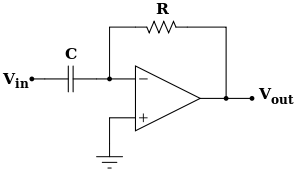
\includegraphics[width=7cm]{../img/bibun_kairo.png}
            \caption{微分回路図. 画像は[1]より引用した.}
        \end{center}
      \end{figure}
    $C$に流れる電流を$I_{i}$とすると,仮想短絡をしているので,次式となる.
      \begin{equation}
        I_{i} = \frac{dQ}{dt} = C_{i}\frac{dV_{i}}{dt}.
      \end{equation}
    出力電圧$V_{o}$は$R_{f}$での電圧降下に等しいので,$V_{o}$は次式のようになる.
      \begin{equation}
        V_{o} = - I_{i} R_{f} = - C_{i} R_{f} \frac{dV_{i}}{dt}.
      \end{equation}
    このように,$V_{o}$は,入力電圧$V_{i}$を微分した値に比例する出力となる. また,
    このままでは動作が不安定であるので,実際には$C$に直列に$R_{i}$を,$R$に
    並列に$C_{f}$を入れた回路にする.微分器として安定な上限の周波数$f_{s}$は次式で求まる.
      \begin{equation}
        f_{s} = \frac{1}{2 \pi R_{i} C_{i}}.
      \end{equation}


  \subsection{積分回路}
  % 積分回路
      $R_{i}$を流れる電流を$I_{i}$とすると,仮想短絡をしているので,次式となる
        \begin{equation}
          V_{i} = I_{i} R_{i}.
        \end{equation}  
      また,コンデンサ$C_{f}$の電荷を$Q_{f}$とすると,$Q_{f}$の時間的な増加の割合は
      流れ込む電流$I_{i}$に等しくなるので,次式が成立する.
        \begin{equation}
          \frac{dQ_{f}}{dt} = I_{i}.
        \end{equation}
      積分すると,
        \begin{equation}
          Q_{f} = \int I_{i} dt = \frac{1}{R_{i}} \int V_{i} dt,
        \end{equation}
      となる. $V_{o}$はコンデンサ$C_{f}$による電圧降下量$- \frac{Q_{f}}{C_{f}}$に等しいので,
        \begin{equation}
          V_{o} = - \frac{1}{R_{f}C_{f}} \int V_{i} dt,
        \end{equation}
      となり,入力電圧$V_{i}$を積分した値に比例する出力が得られることがわかる.


\section{方法}
% 方法
    \subsection{実験装置}
        オペアンプ実習装置に,外付けの抵抗,コンデンサなどを接続し,各種アナログ回路を設計し,
        オシロスコープ,任意信号発生器により,その動作を確認する.

    \subsection{方法}
        \begin{enumerate}
          \item 反転増幅回路を作成し,入出力特性,周波数特性を調べる. また,増幅度が異なる回路を設計し,
            その回路の特性を設定する. \\
          \item ローパスおよびはいパスフィルタを作成し,各周波数$f$における電圧増幅度$G$を計測し,
            $f - G$特性を求める.
          \item 微分および積分回路を作成し,入出力特性をオシロスコープで観察し,回路動作を確認する.
        \end{enumerate}
    
    \subsection{反転増幅回路の入出力特性}
        \begin{enumerate}
          \item 入力電圧の測定端子は次の通りである. \\
            入力電圧: TB11($V_{in}$),TB14(GND) \\
            出力電圧: TV15($V_{out}$),TB16(GND) \\
          \item 試験用DC電圧発生部と増幅回路を図2のように接続した. \\
          \item 増幅回路を次のように設定した. \\
            R$_{11}$: 10$k\Omega$,R$_{12}$: 開放,R$_{13}$: 開放, \\
            R$_{14}$: 10$k\Omega$,R$_{15}$: 5,1$k\Omega$,R$_{16}$: 10$k\Omega$
          \item 出力電圧$V_{out}$が0Vであることをオシロスコープで確認する.
          \item 試験用DC電圧発生部の-3V - +3V まで変えて,入出力電圧をオシロスコープで観測する.
          \item 電圧増幅度$A$が-10となるような回路を設計し,同様に実習する.
        \end{enumerate}


        \begin{figure}[]
          \begin{center}
              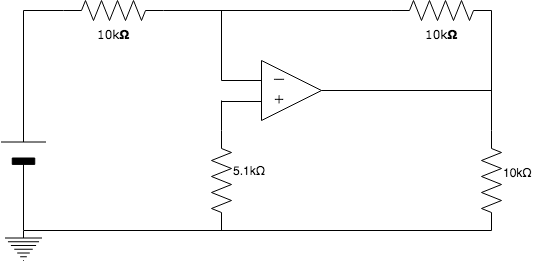
\includegraphics[width=7cm]{../img/hi_hanten_zoufuku_kairo.png}
              \caption{非反転増幅回路の結線法.}
          \end{center}
        \end{figure}


    \subsection{反転増幅回路の周波数特性および位相}
        \begin{enumerate}
            \item 3.3節の(6)が完了した状態にする. \\
            \item 試験用DCの電圧発生部の接続を外し,信号発生器をTB11,TB14に接続する. \\
            \item オシロスコープを$V_{in}$および$V_{out}$に接続する.
            \item オシロスコープを見ながら,信号発生器の出力を1.2V$_{p.p}$,100Hzに設定する. \\
            \item 周波数を100Hzから1MHzまで変える \\
              \begin{enumerate}
                \item 出力電圧$V_{out}$の振幅と位相がどのように変わるかをオシロスコープで観測する. \\
                \item 低周波では入出力波形の位相差が180度であることをオシロスコープで確認する. \\
              \end{enumerate}
            \item 5.のデータから周波数$f$電圧増幅度$G$の関係を片対数グラフにする.
        \end{enumerate}

    \subsection{ローパスフィルタ回路}
        \begin{enumerate}
          \item アクティブフィルタ回路において,図3に示すローパスフィルタ回路を作成する. \\
          \item 作成した回路の$Q$および$\omega_{0},f_{0}$を計算する. \\
          \item 信号発生器の出力を1.2V$_{p-p}$に設定し,波形と周波数を以下のようにする. \\
              \begin{enumerate}
                  \item 5kHzの方形波を入力とした際の出力波形をオシロスコープで観測する. \\
                  \item $f_{0}$を含む20パターン程度の周波数の正弦波を入力し,入力電圧および出力電圧を計測する.
              \end{enumerate}
          \item 電圧増幅度$G$に換算して$f-G$特性をグラフに表す.
        \end{enumerate}

        \begin{figure}[]
          \begin{center}
              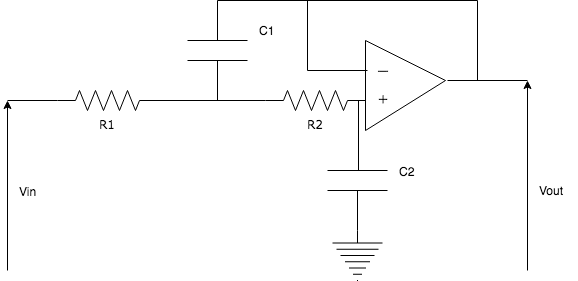
\includegraphics[width=7cm]{../img/ro-pasu.png}
              \caption{ローパスフィルタの回路図.}
          \end{center}
        \end{figure}
      
    \subsection{ハイパスフィルタ回路}
        \begin{enumerate}
          \item アクティブフィルタ回路において,図4に示す示すハイパスフィルタ回路を作成する. \\
          \item 作成した回路の$Q$および,$\omega_{0},f_{0}$を計算により求める. \\
          \item 信号発生器の出力を1.2V$_{p-p}$に設定し,波形と周波数を以下のように変える. \\
              \begin{enumerate}
                  \item 5kHzの方形波を入力した際の出力波形をオシロスコープで観測する. \\
                  \item $f_{0}$を含む20パターン程度の周波数の正弦波を入力し,入力電圧および出力電圧を計測する. \\
              \end{enumerate}
          \item 電圧増幅度$G$に換算して$f-G$特性をグラフに表す.
        \end{enumerate}

        \begin{figure}[]
          \begin{center}
              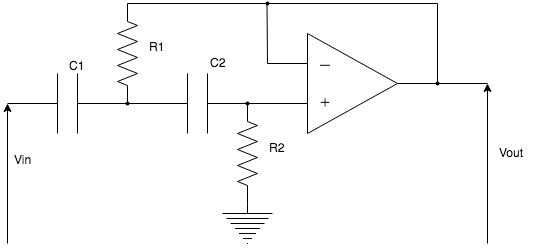
\includegraphics[width=7cm]{../img/highpass.png}
              \caption{ハイフィルタの回路図.}
          \end{center}
        \end{figure}
    
    \subsection{微分回路}
        \begin{enumerate}
          \item 図5に示す微分回路を作成する. \\
          \item 微分器として安定な上限の周波数$f_{s}$を計算により求める. \\
          \item 信号発生器の出力を1V$_{p-p}$の方形波に設定し,3通りの周波数$(f=f_{s},f > f_{s},f < f_{s})$とした際の出力波形をオシロスコープで観測する.
          
        \end{enumerate}

        \begin{figure}[]
          \begin{center}
              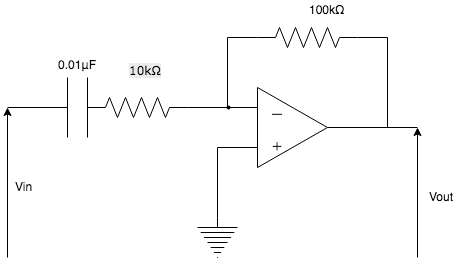
\includegraphics[width=7cm]{../img/bibunkairo.png}
              \caption{微分回路の回路図.}
          \end{center}
        \end{figure}
    
    \subsection{積分回路}
        \begin{enumerate}
          \item 図6に示す積分回路を作成する. \\
          \item 積分器として安定な下限の周波数$f_{p}$を計算により求める. \\
          \item 信号発生器の出力を1V$_{p-p}$の方形波に設定し,3通りの周波数$(f=f_{s},f > f_{s},f < f_{s})$とした際の出力波形をオシロスコープで観測する.
        \end{enumerate}


        \begin{figure}[]
          \begin{center}
              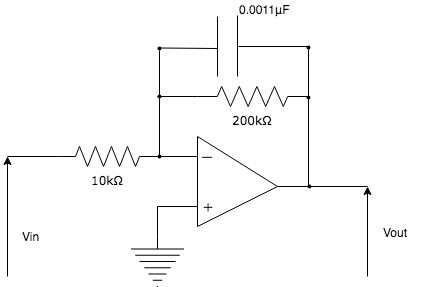
\includegraphics[width=7cm]{../img/sekibun_kairo_.png}
              \caption{積分回路の回路図.}
          \end{center}
        \end{figure}


\section{結果}
% 結果
    \subsection{反転増幅回路($A=-1$)の入出力特性}
        測定結果を表2,図7に示した. 


        \begin{table}[H]
          \centering
          \footnotesize
          \caption{反転増幅回路の測定結果.}
          \label{opeanpu_risouteki_tokusei}
          \begin{tabular}{lll} \hline
            入力[V] &	出力[V] & 電圧増幅度 $A$  \\ \hline

-2.98&3.04&1.020134228 \\
-2.53&2.6&1.027667984 \\
-1.98&2.07&1.045454545 \\
-1.51&1.6&1.059602649 \\
-1.05&1.15&1.095238095 \\
-0.49&0.57&1.163265306 \\
0.000002&0.08&40000 \\
0.49&-0.42&0.8571428571 \\
1&-0.92&0.92 \\
1.53&-1.45&0.9477124183 \\
2.02&-1.93&0.9554455446 \\
2.52&-2.42&0.9603174603 \\
3.03&-2.92&0.9636963696 \\ \hline
            
          \end{tabular}
        \end{table}

        \begin{figure}[]
          \begin{center}
              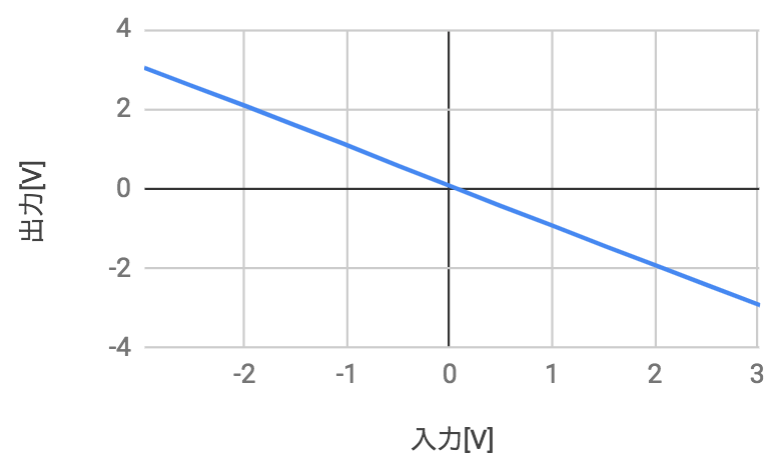
\includegraphics[width=7cm]{../img/hantenzoufuku_result_1.png}
              \caption{反転増幅回路の測定結果.}
          \end{center}
        \end{figure}

    \subsection{反転増幅回路の増幅度を変化($A=-10$)させた時の入出力特性}
        測定結果を表3,図8に示した. 
        

                  \begin{table}[H]
                    \centering
                    \footnotesize
                    \caption{反転増幅回路の測定結果.}
                    \label{opeanpu_risouteki_tokusei}
                    \begin{tabular}{lll} \hline
                      入力[V] &出力[V] & 電圧増幅率$A$ \\ \hline
                      -2.98&14.7&4.932885906 \\
                      -2.98&14.7&4.932885906 \\
                      -2.98&14.7&4.932885906 \\
                      -1.52&14.7&9.671052632 \\
                      -1&11&11 \\
                      -0.53&6.43&12.13207547 \\
                      0&1& - \\
                      0.51&-4.1&8.039215686 \\
                      0.99&-9&9.090909091 \\
                      1.52&-12.4&8.157894737 \\
                      2.03&-12.4&6.108374384 \\
                      2.46&-12.4&5.040650407 \\
                      3&-12.4&4.133333333 \\ \hline
                    \end{tabular}
                  \end{table}

                  \begin{figure}[]
                    \begin{center}
                        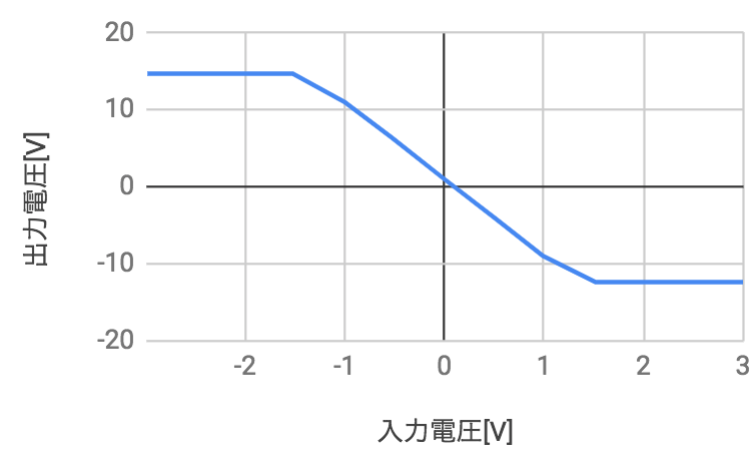
\includegraphics[width=7cm]{../img/hantenzoufuku_result_2.png}
                        \caption{反転増幅回路の測定結果.}
                    \end{center}
                  \end{figure}

      \subsection{反転増幅回路の周波数特性}
          測定結果を表4,図9,10に示した. 位相差は$2\pi * (周波数Hz * 位相差s)$で求めた.

          \begin{table*}[t]
            \centering
            \footnotesize
            \caption{反転増幅回路の測定結果.}
            \label{opeanpu_risouteki_tokusei}
            \begin{tabular}{llllll} \hline
周波数$f$kHz	& 入力V$_{p-p}$	& 出力電圧V$_{p_p}$	& 位相差μs	& 位相差度	& 電圧増幅度dB \\ \hline
0.1& 1.22& 11.6& 0.005& 3.141592654& 19.56196317 \\
0.5& 1.2& 11.6& 0.001& 3.141592654& 19.70553486 \\
1& 1.2& 11.6& 0.0005& 3.141592654& 19.70553486 \\
5& 1.22& 12& 0.0001& 3.141592654& 19.85642831 \\
10& 1.22& 12& 0.00005& 3.141592654& 19.85642831 \\
20& 1.22& 11.5& 0.000026& 3.26725636& 19.48676019 \\
30& 1.24& 11& 0.0000188& 3.543716513& 18.95942 \\
40& 1.23& 10.6& 0.0000148& 3.719645702& 18.70801508 \\
50& 1.22& 10& 0.000012& 3.769911184& 18.27280339 \\
60& 1.22& 9.4& 0.0000102& 3.845309408& 17.73536046 \\
70& 1.23& 8.8& 0.000009& 3.958406744& 17.09155121 \\
80& 1.22& 8.2& 0.000008& 4.021238597& 16.54908043 \\
90& 1.22& 7.8& 0.0000074& 4.184601415& 16.11469544 \\
100& 1.22& 7.4& 0.0000068& 4.272566009& 15.65743778 \\
200& 1.22& 4.6& 0.0000036& 4.523893421& 11.52796002 \\
300& 1.24& 2.9& 0.00000248& 4.674689869& 7.379526255 \\
400& 1.24& 2.2& 0.00000196& 4.926017281& 4.980019913 \\
500& 1.24& 1.8& 0.0000016& 5.026548246& 3.237016399 \\
600& 1.22& 1.52& 0.00000132& 4.976282763& 1.909675145 \\
700& 1.22& 1.2& 0.00000116& 5.101946469& -0.1435716925 \\
800& 1.24& 1.06& 0.00000104& 5.227610176& -1.362316398 \\
900& 1.22& 0.95& 0.00000094& 5.31557477& -2.172724508 \\
1000& 1.22& 0.82& 0.00000088& 5.52920307& -3.450919566 \\ \hline

            \end{tabular}
          \end{table*}

          \begin{figure}[]
            \begin{center}
                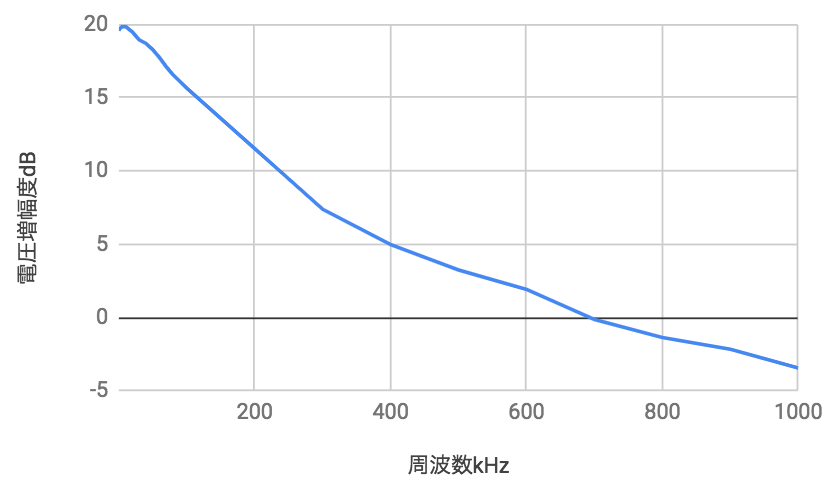
\includegraphics[width=7cm]{../img/syuuhasuu_denatuzoufuku.png}
                \caption{周波数Hzと電圧増幅度dBの関係.}
            \end{center}
          \end{figure}

          \begin{figure}[]
            \begin{center}
                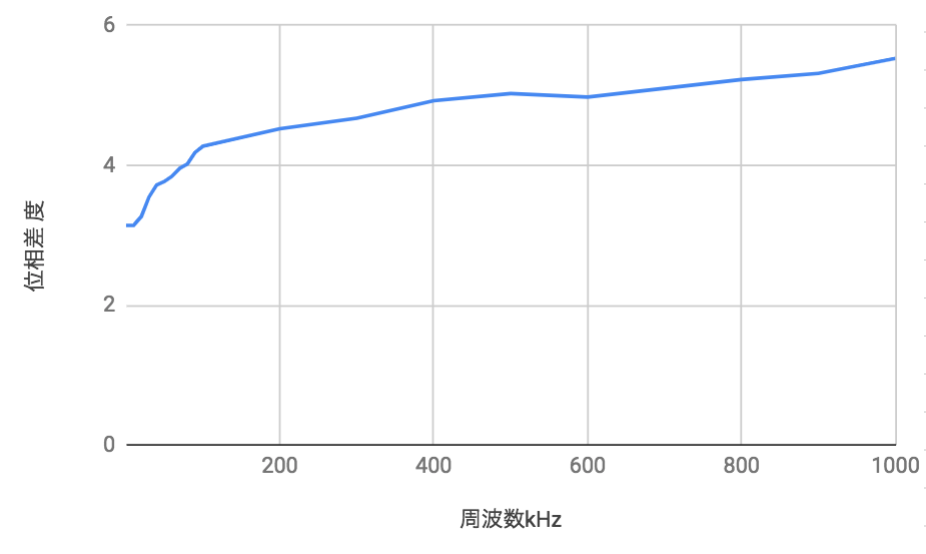
\includegraphics[width=7cm]{../img/syuuhasuu_isousa_do.png}
                \caption{周波数Hzと位相差 度の関係.}
            \end{center}
          \end{figure}



      \subsection{ローパスフィルタの周波数特性と波形}
           測定結果を表5,6,図11,12に示した.

           \begin{table}[H]
            \centering
            \footnotesize
            \caption{ローパスフィルタの抵抗と静電容量の値.}
            \label{opeanpu_risouteki_tokusei}
            \begin{tabular}{llllll} \hline
              $R_{1} k \Omega$ & $R_{2} k \Omega$& $C_{1} \mu F$& $C_{2} \mu F$& $f_{0} Hz$ & $Q$ \\ \hline
              10& 220& 0.0022& 0.0011& 2181.228& 0.288 \\ \hline
            \end{tabular}
          \end{table}

          \begin{table*}[t]
            \centering
            \footnotesize
            \caption{ローパスフィルタの測定結果.}
            \label{opeanpu_risouteki_tokusei}
          \begin{tabular}{lllll} \hline

              $f$Hz& 入力電圧$V_{i}$ mV& 出力電圧 $V_{o}$ mV& log(A)& 20logA dB \\ \hline
              10& 960& 960& 2.302585093& 0 \\
              30& 980& 960& 3.401197382& -0.1790968531 \\
              100& 980& 960& 4.605170186& -0.1790968531 \\
              200& 980& 920& 5.298317367& -0.5487649669 \\
              300& 980& 900& 5.703782475& -0.7396713251 \\
              400& 980& 840& 5.991464547& -1.338935793 \\
              600& 980& 760& 6.396929655& -2.208249668 \\
              800& 980& 660& 6.684611728& -3.433642803 \\
              1000& 980& 580& 6.907755279& -4.555961643 \\
              1200& 980& 520& 7.090076836& -5.504454641 \\
              1400& 980& 480& 7.244227516& -6.199696766 \\
              1600& 980& 420& 7.377758908& -7.359535706 \\
              1800& 980& 380& 7.495541944& -8.228849582 \\
              2000& 1000& 344& 7.60090246& -9.268831149 \\
              2181& 980& 320& 7.687538766& -9.721521947 \\
              2400& 1000& 296& 7.783224016& -10.57416578 \\
              2600& 1000& 264& 7.863266724& -11.56792146 \\
              2800& 1000& 248& 7.937374696& -12.11096638 \\
              3000& 1040& 232& 8.006367568& -13.03090709 \\
              4000& 1020& 240& 8.29404964& -12.5677786 \\
              5000& 1040& 200& 8.517193191& -14.32006687 \\
              10000& 1020& 140& 9.210340372& -17.24944272 \\
              30000& 1020& 100& 10.30895266& -20.17200344 \\ \hline

            \end{tabular}
          \end{table*}


          \begin{figure}[]
            \begin{center}
                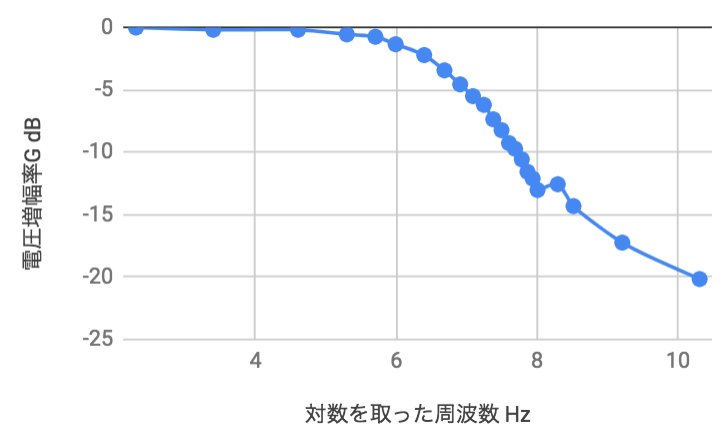
\includegraphics[width=7cm]{../img/low_pass_result.png}
                \caption{ローパスフィルタ回路の周波数と電圧増幅率の関係.}
            \end{center}
          \end{figure}
          
          \begin{figure}[]
            \begin{center}
                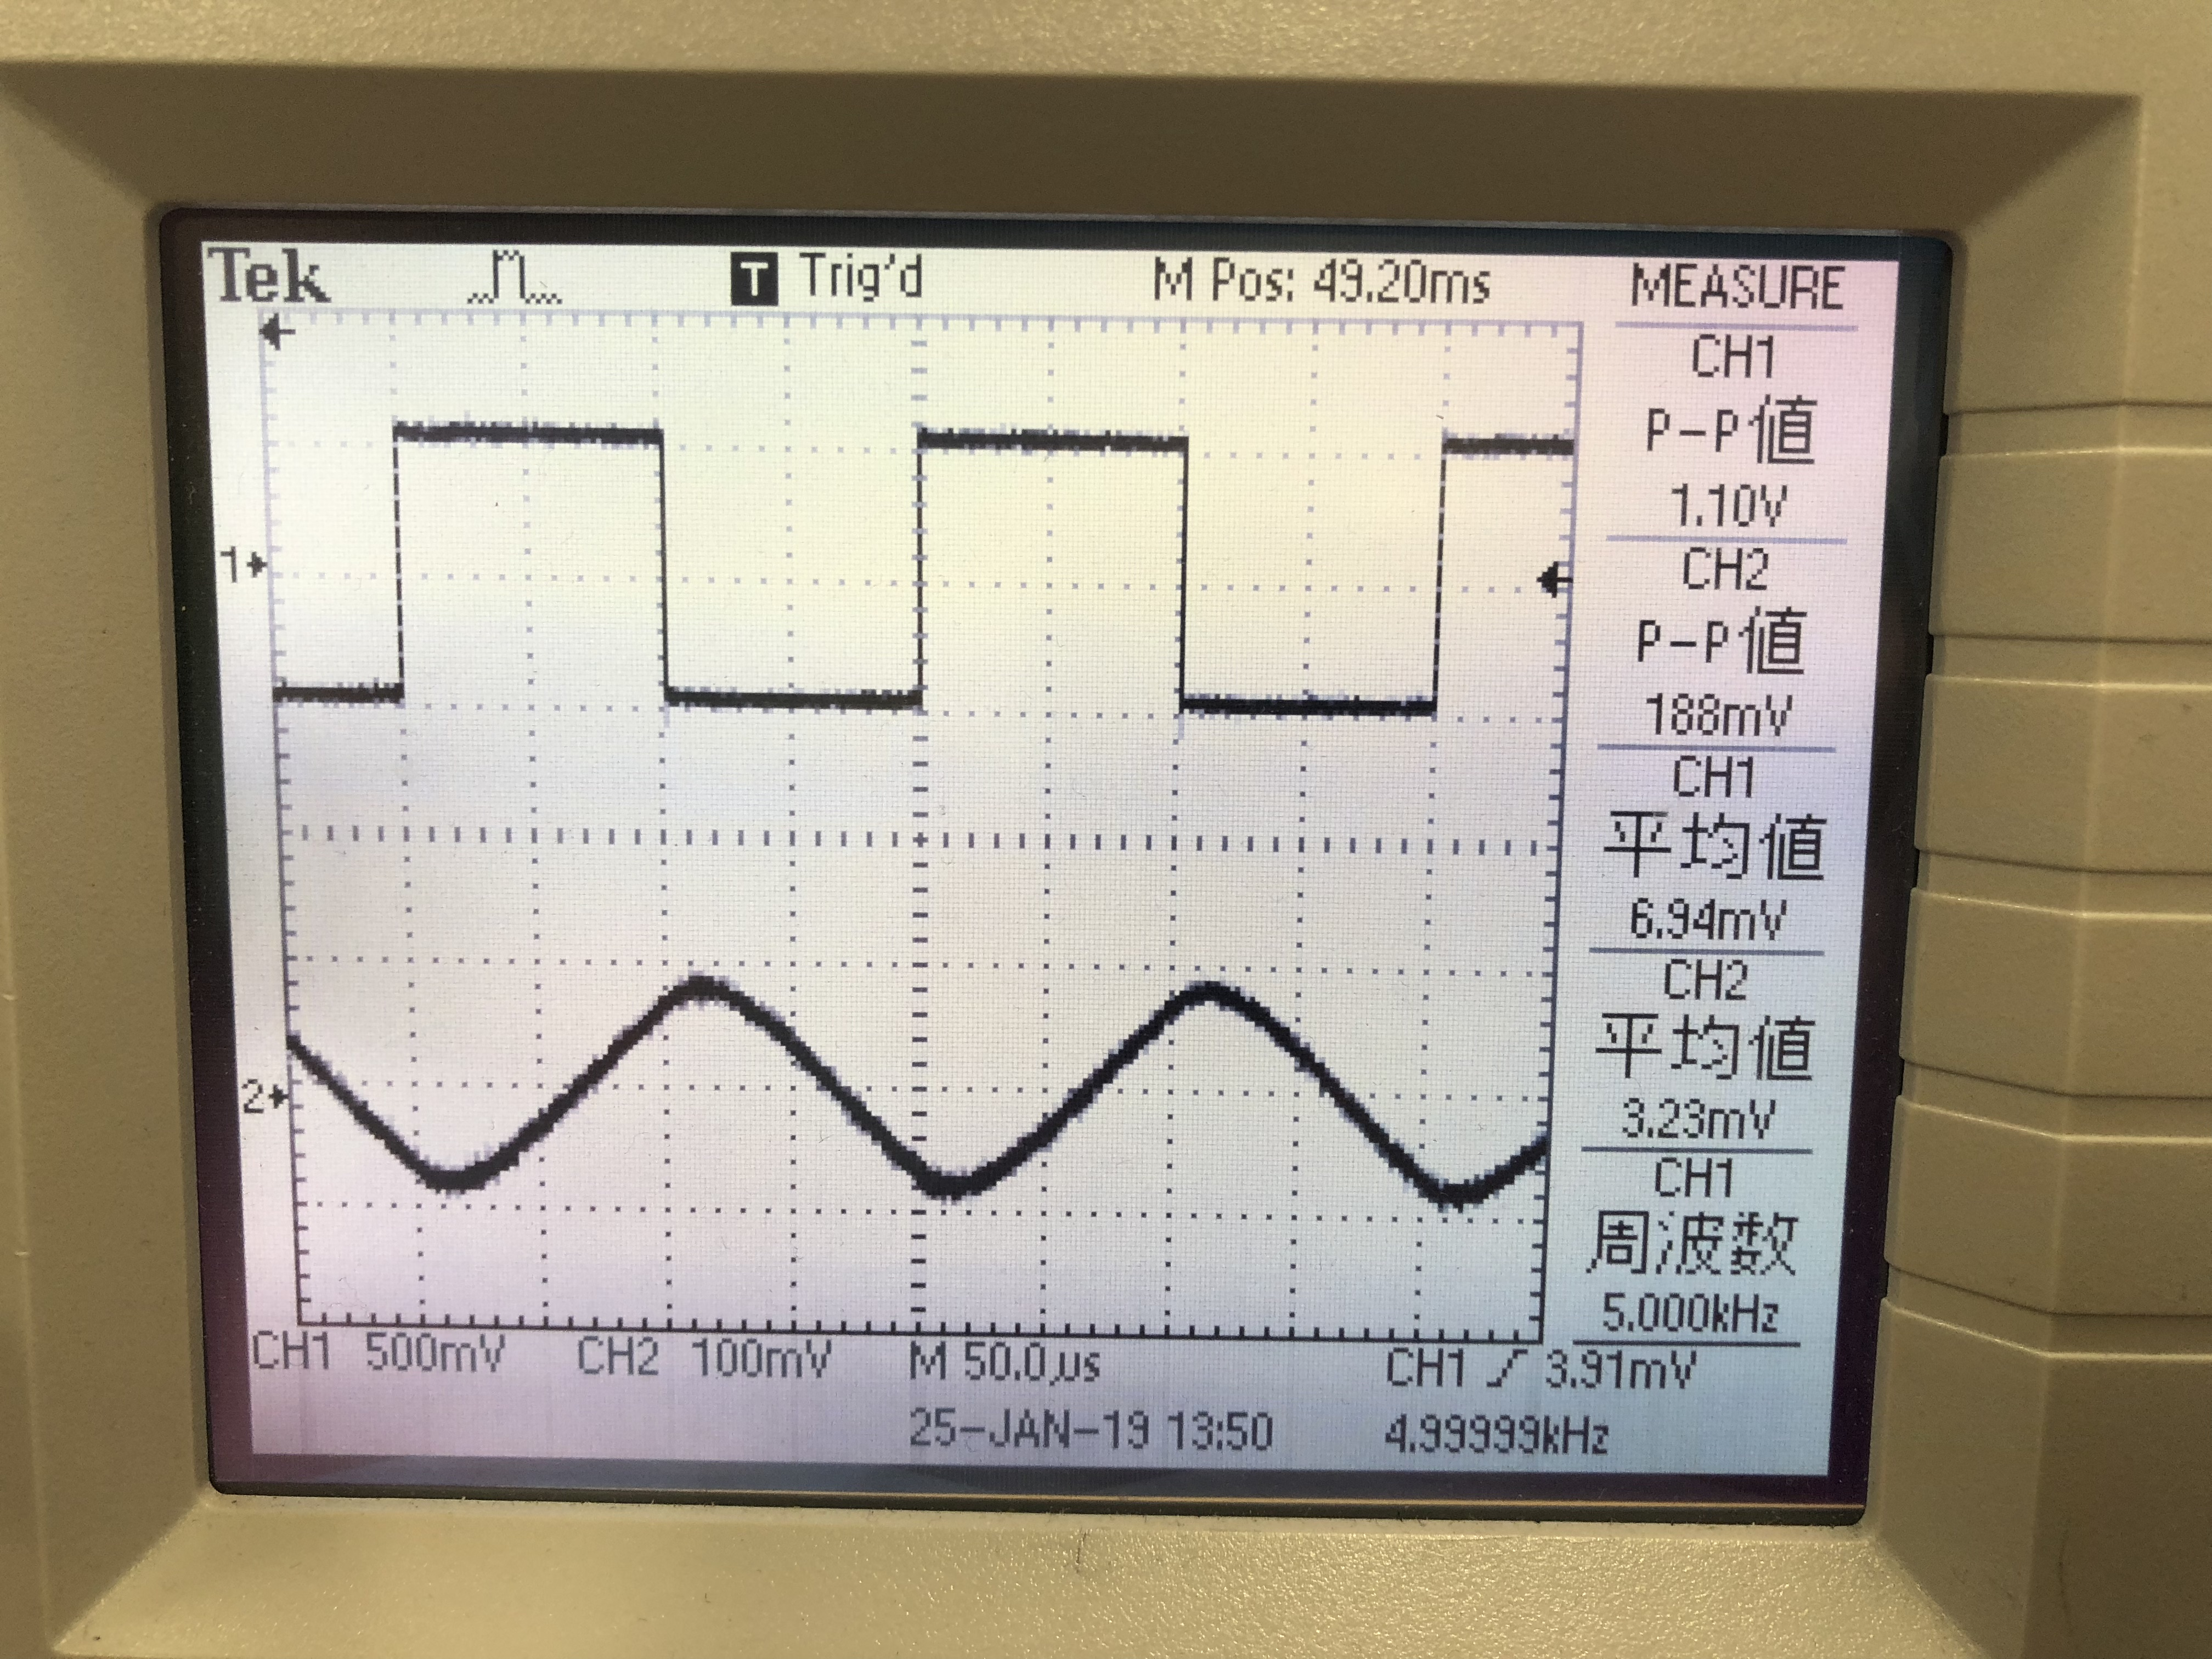
\includegraphics[width=7cm]{../img/result_low_pass_vis.jpg}
                \caption{ローパスフィルタのオシロスコープによる可視化結果.}
            \end{center}
          \end{figure}
          

      \subsection{ハイパスフィルタの周波数特性と波形}
          結果を表7,8,図13,14に示した.

          \begin{table}[H]
            \centering
            \footnotesize
            \caption{ハイパスの抵抗と静電容量の値.}
            \label{opeanpu_risouteki_tokusei}
            \begin{tabular}{llllll} \hline
              $R_{1} k \Omega$ & $R_{2} k \Omega$& $C_{1} \mu F$& $C_{2} \mu F$& $f_{0} Hz$ & $Q$ \\ \hline
              220	& 10	& 0.0022	& 0.0011	& 2181.228	& 0.101 \\ \hline
            \end{tabular}
          \end{table}


          \begin{table*}[t]
            \centering
            \footnotesize
            \caption{ローパスフィルタの測定結果.}
            \label{opeanpu_risouteki_tokusei}
          \begin{tabular}{lllll} \hline

                  $f$Hz& 入力電圧$V_{i}$ mV& 出力電圧 $V_{o}$ mV& log(A)& 20logA dB \\ \hline
                  10& 960& 60& 2.302585093& -24.08239965 \\
                  30& 960& 60& 3.401197382& -24.08239965 \\
                  100& 940& 60& 4.605170186& -23.89953206 \\
                  200& 940& 60& 5.298317367& -23.89953206 \\
                  300& 940& 60& 5.703782475& -23.89953206 \\
                  400& 960& 60& 5.991464547& -24.08239965 \\
                  600& 940& 40& 6.396929655& -27.42135725 \\
                  800& 940& 80& 6.684611728& -21.40075733 \\
                  1000& 960& 100& 6.907755279& -19.64542466 \\
                  1200& 960& 100& 7.090076836& -19.64542466 \\
                  1400& 960& 100& 7.244227516& -19.64542466 \\
                  1600& 960& 120& 7.377758908& -18.06179974 \\
                  1800& 960& 120& 7.495541944& -18.06179974 \\
                  2000& 960& 140& 7.60090246& -16.72286395 \\
                  2181& 960& 140& 7.687538766& -16.72286395 \\
                  2400& 960& 140& 7.783224016& -16.72286395 \\
                  2600& 960& 160& 7.863266724& -15.56302501 \\
                  2800& 960& 160& 7.937374696& -15.56302501 \\
                  3000& 960& 160& 8.006367568& -15.56302501 \\
                  4000& 960& 200& 8.29404964& -13.62482475 \\
                  5000& 980& 240& 8.517193191& -12.22029668 \\
                  6000& 1000& 340& 8.699514748& -9.370421659 \\
                  7000& 1000& 360& 8.853665428& -8.873949985 \\
                  8000& 1000& 390& 8.987196821& -8.178707859 \\
                  9000& 1020& 420& 9.104979856& -7.707017627 \\
                  9500& 1000& 440& 9.159047078& -7.13094647 \\
                  10000& 960& 460& 9.210340372& -6.390268027 \\
                  11000& 1000& 480& 9.305650552& -6.375175252 \\
                  11500& 1000& 490& 9.350102314& -6.196078399 \\
                  12000& 1000& 520& 9.392661929& -5.679933127 \\
                  13000& 1000& 540& 9.472704636& -5.352124804 \\
                  14000& 1000& 570& 9.546812609& -4.882502887 \\
                  16000& 1000& 600& 9.680344001& -4.436974992 \\
                  17000& 1020& 620& 9.740968623& -4.324169645 \\
                  18000& 1000& 640& 9.798127037& -3.87640052 \\
                  19000& 1000& 660& 9.852194258& -3.609121289 \\
                  20000& 1000& 680& 9.903487553& -3.349821746 \\
                  25000& 1000& 740& 10.1266311& -2.615365605 \\
                  30000& 1000& 800& 10.30895266& -1.93820026 \\
                  40000& 1000& 840& 10.59663473& -1.514414279 \\
                  50000& 1000& 900& 10.81977828& -0.9151498112 \\
                  60000& 1020& 920& 11.00209984& -0.8962468883 \\
                  70000& 1000& 930& 11.15625052& -0.6303410289 \\
                  80000& 1000& 940& 11.28978191& -0.537442928 \\
                  90000& 1000& 960& 11.40756495& -0.3545753392 \\
                  100000& 1000& 960& 11.51292546& -0.3545753392 \\
                  150000& 1000& 960& 11.91839057& -0.3545753392 \\ \hline

            \end{tabular}
          \end{table*}


          \begin{figure}[]
            \begin{center}
                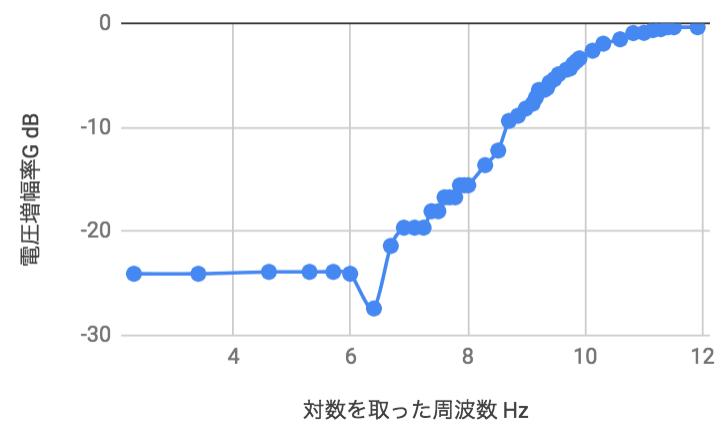
\includegraphics[width=7cm]{../img/high_result.png}
                \caption{ハイパスフィルタ回路の周波数と電圧増幅率の関係.}
            \end{center}
          \end{figure}

          \begin{figure}[]
            \begin{center}
                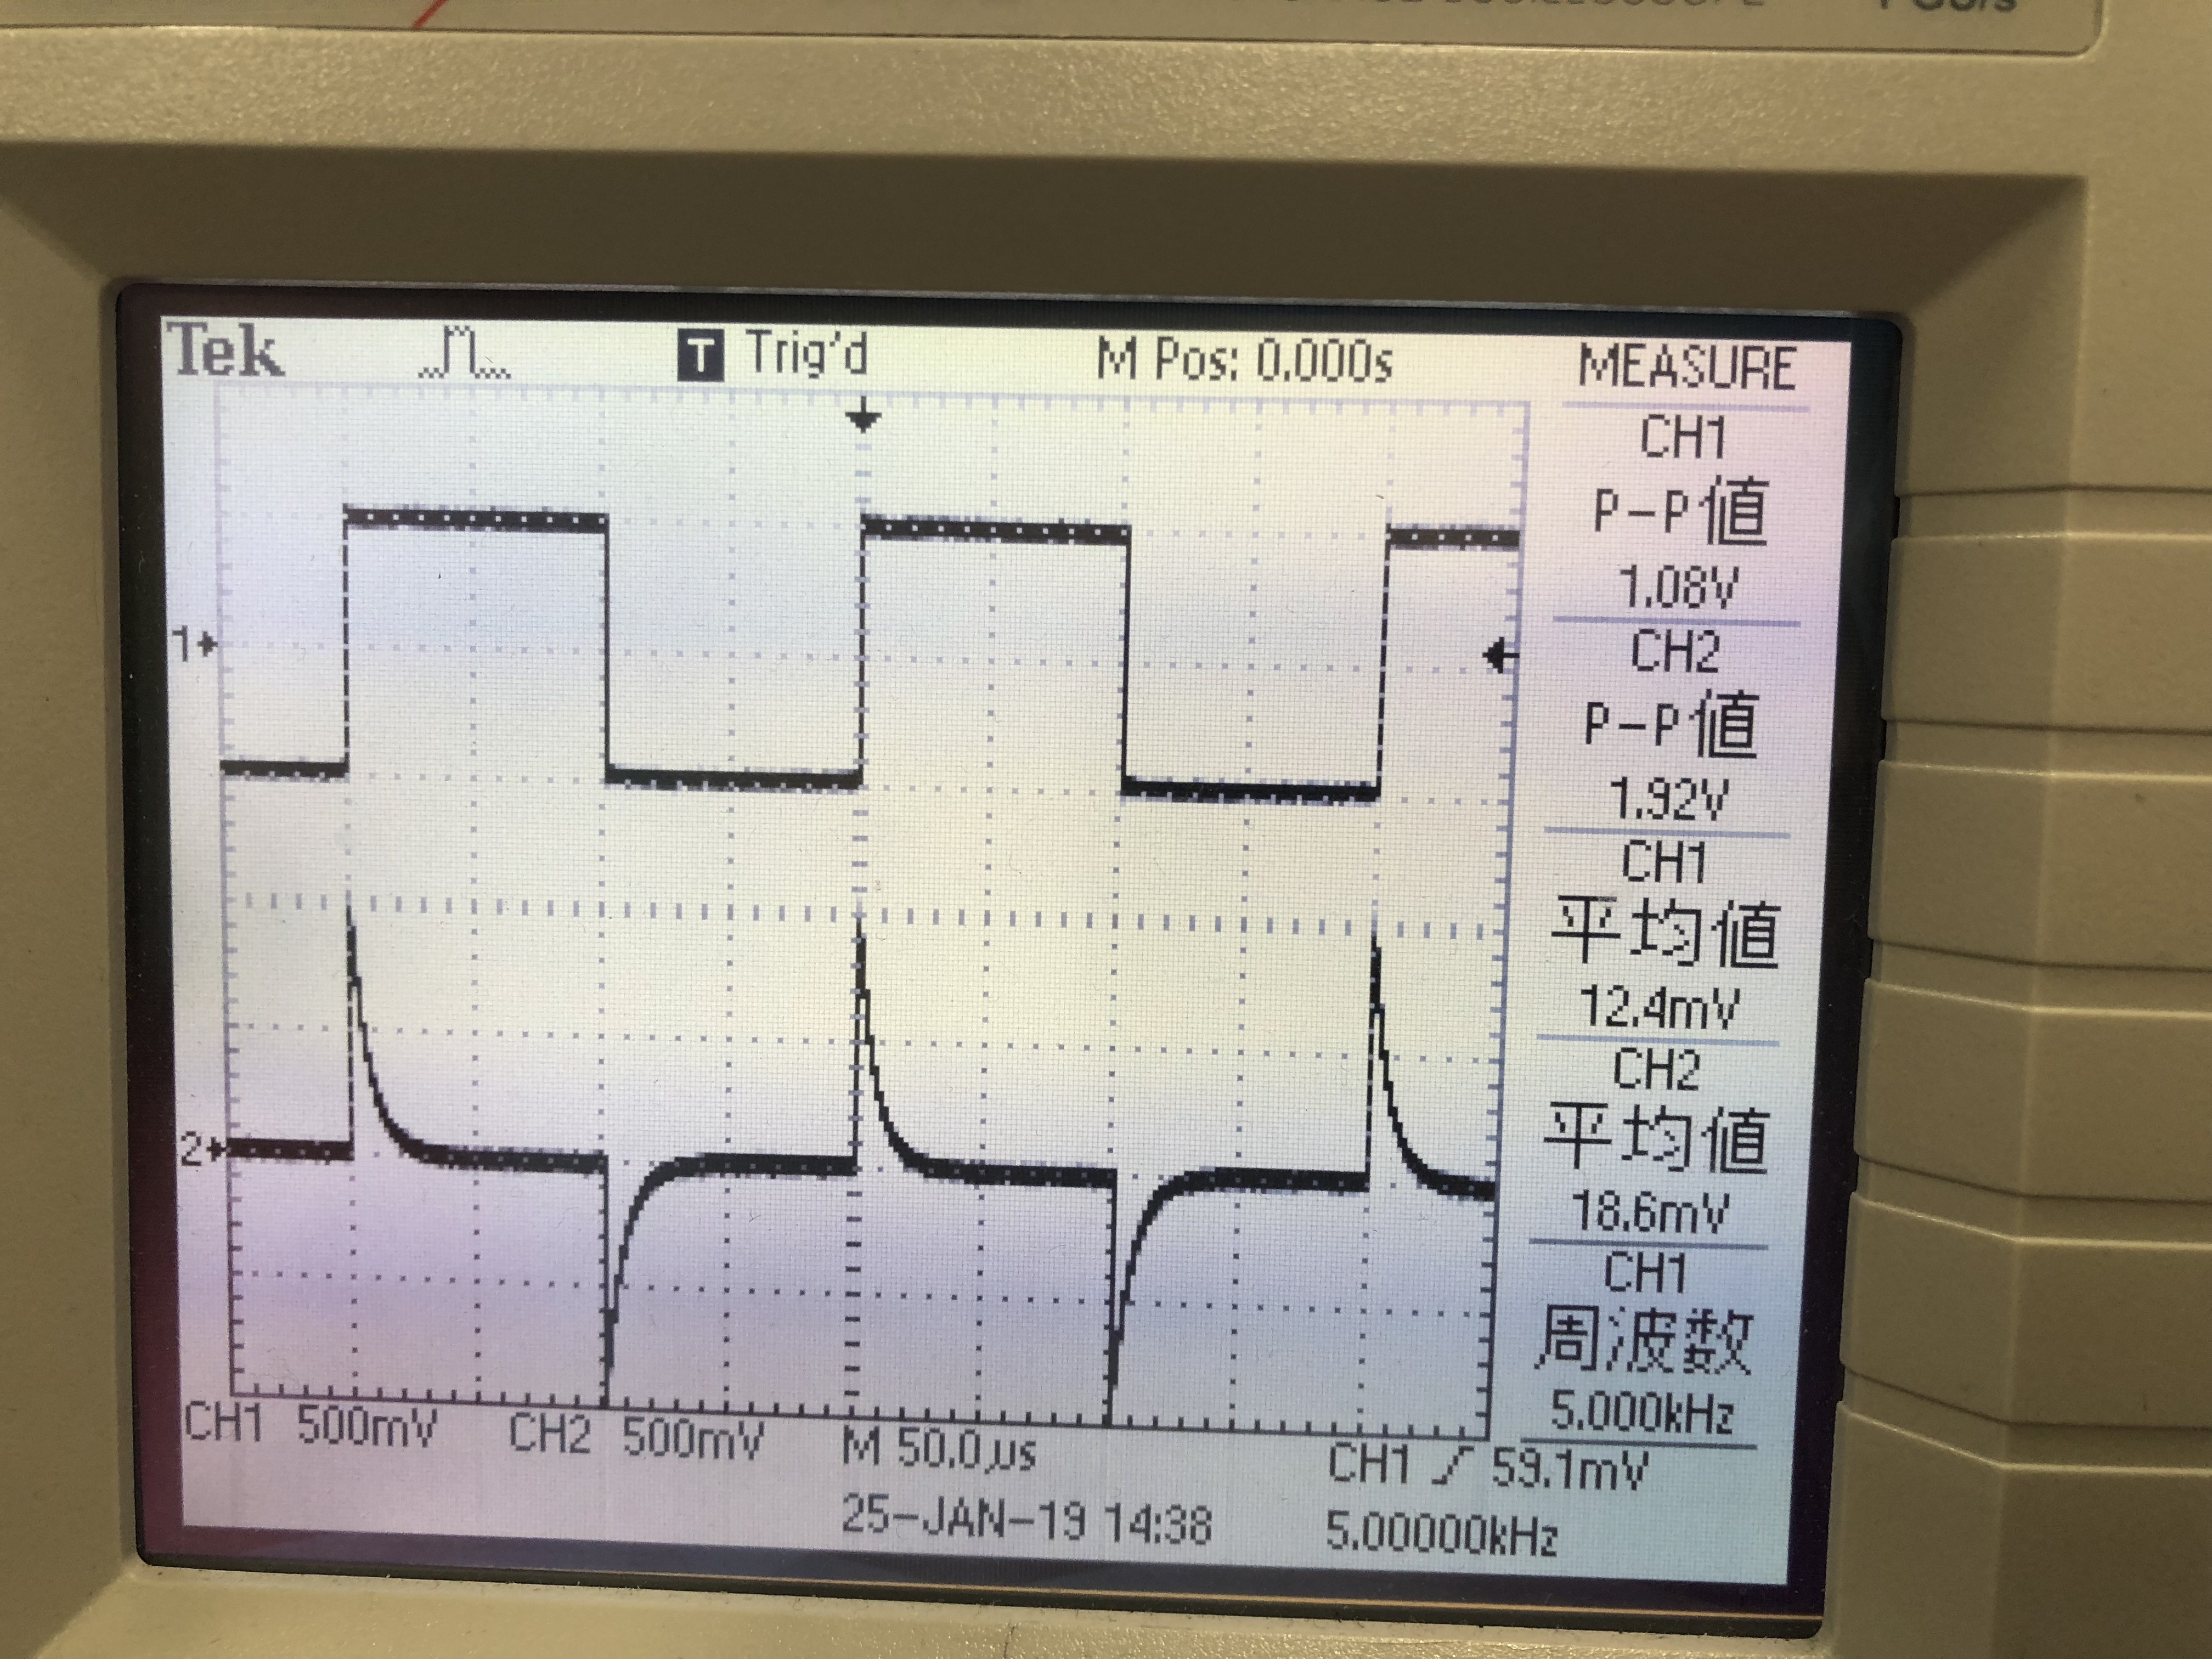
\includegraphics[width=7cm]{../img/result_high_pass_vis.jpg}
                \caption{ハイパスフィルタのオシロスコープによる可視化結果.}
            \end{center}
          \end{figure}


      \subsection{微分回路}
          結果を表8,図15,16,17に示した.



          \begin{table}[H]
            \centering
            \footnotesize
            \caption{微分回路の抵抗,静電容量,$f_{s}$の値.}
            \label{opeanpu_risouteki_tokusei}
            \begin{tabular}{llll} \hline
              $C_{1} \mu F$ & $R_{1} k \Omega$& $R_{2} k \Omega$& $f_{0} Hz$ \\ \hline
              0.01&	10&	100&	1591.549431 \\ \hline
            \end{tabular}
          \end{table}


          \begin{figure}[]
            \begin{center}
                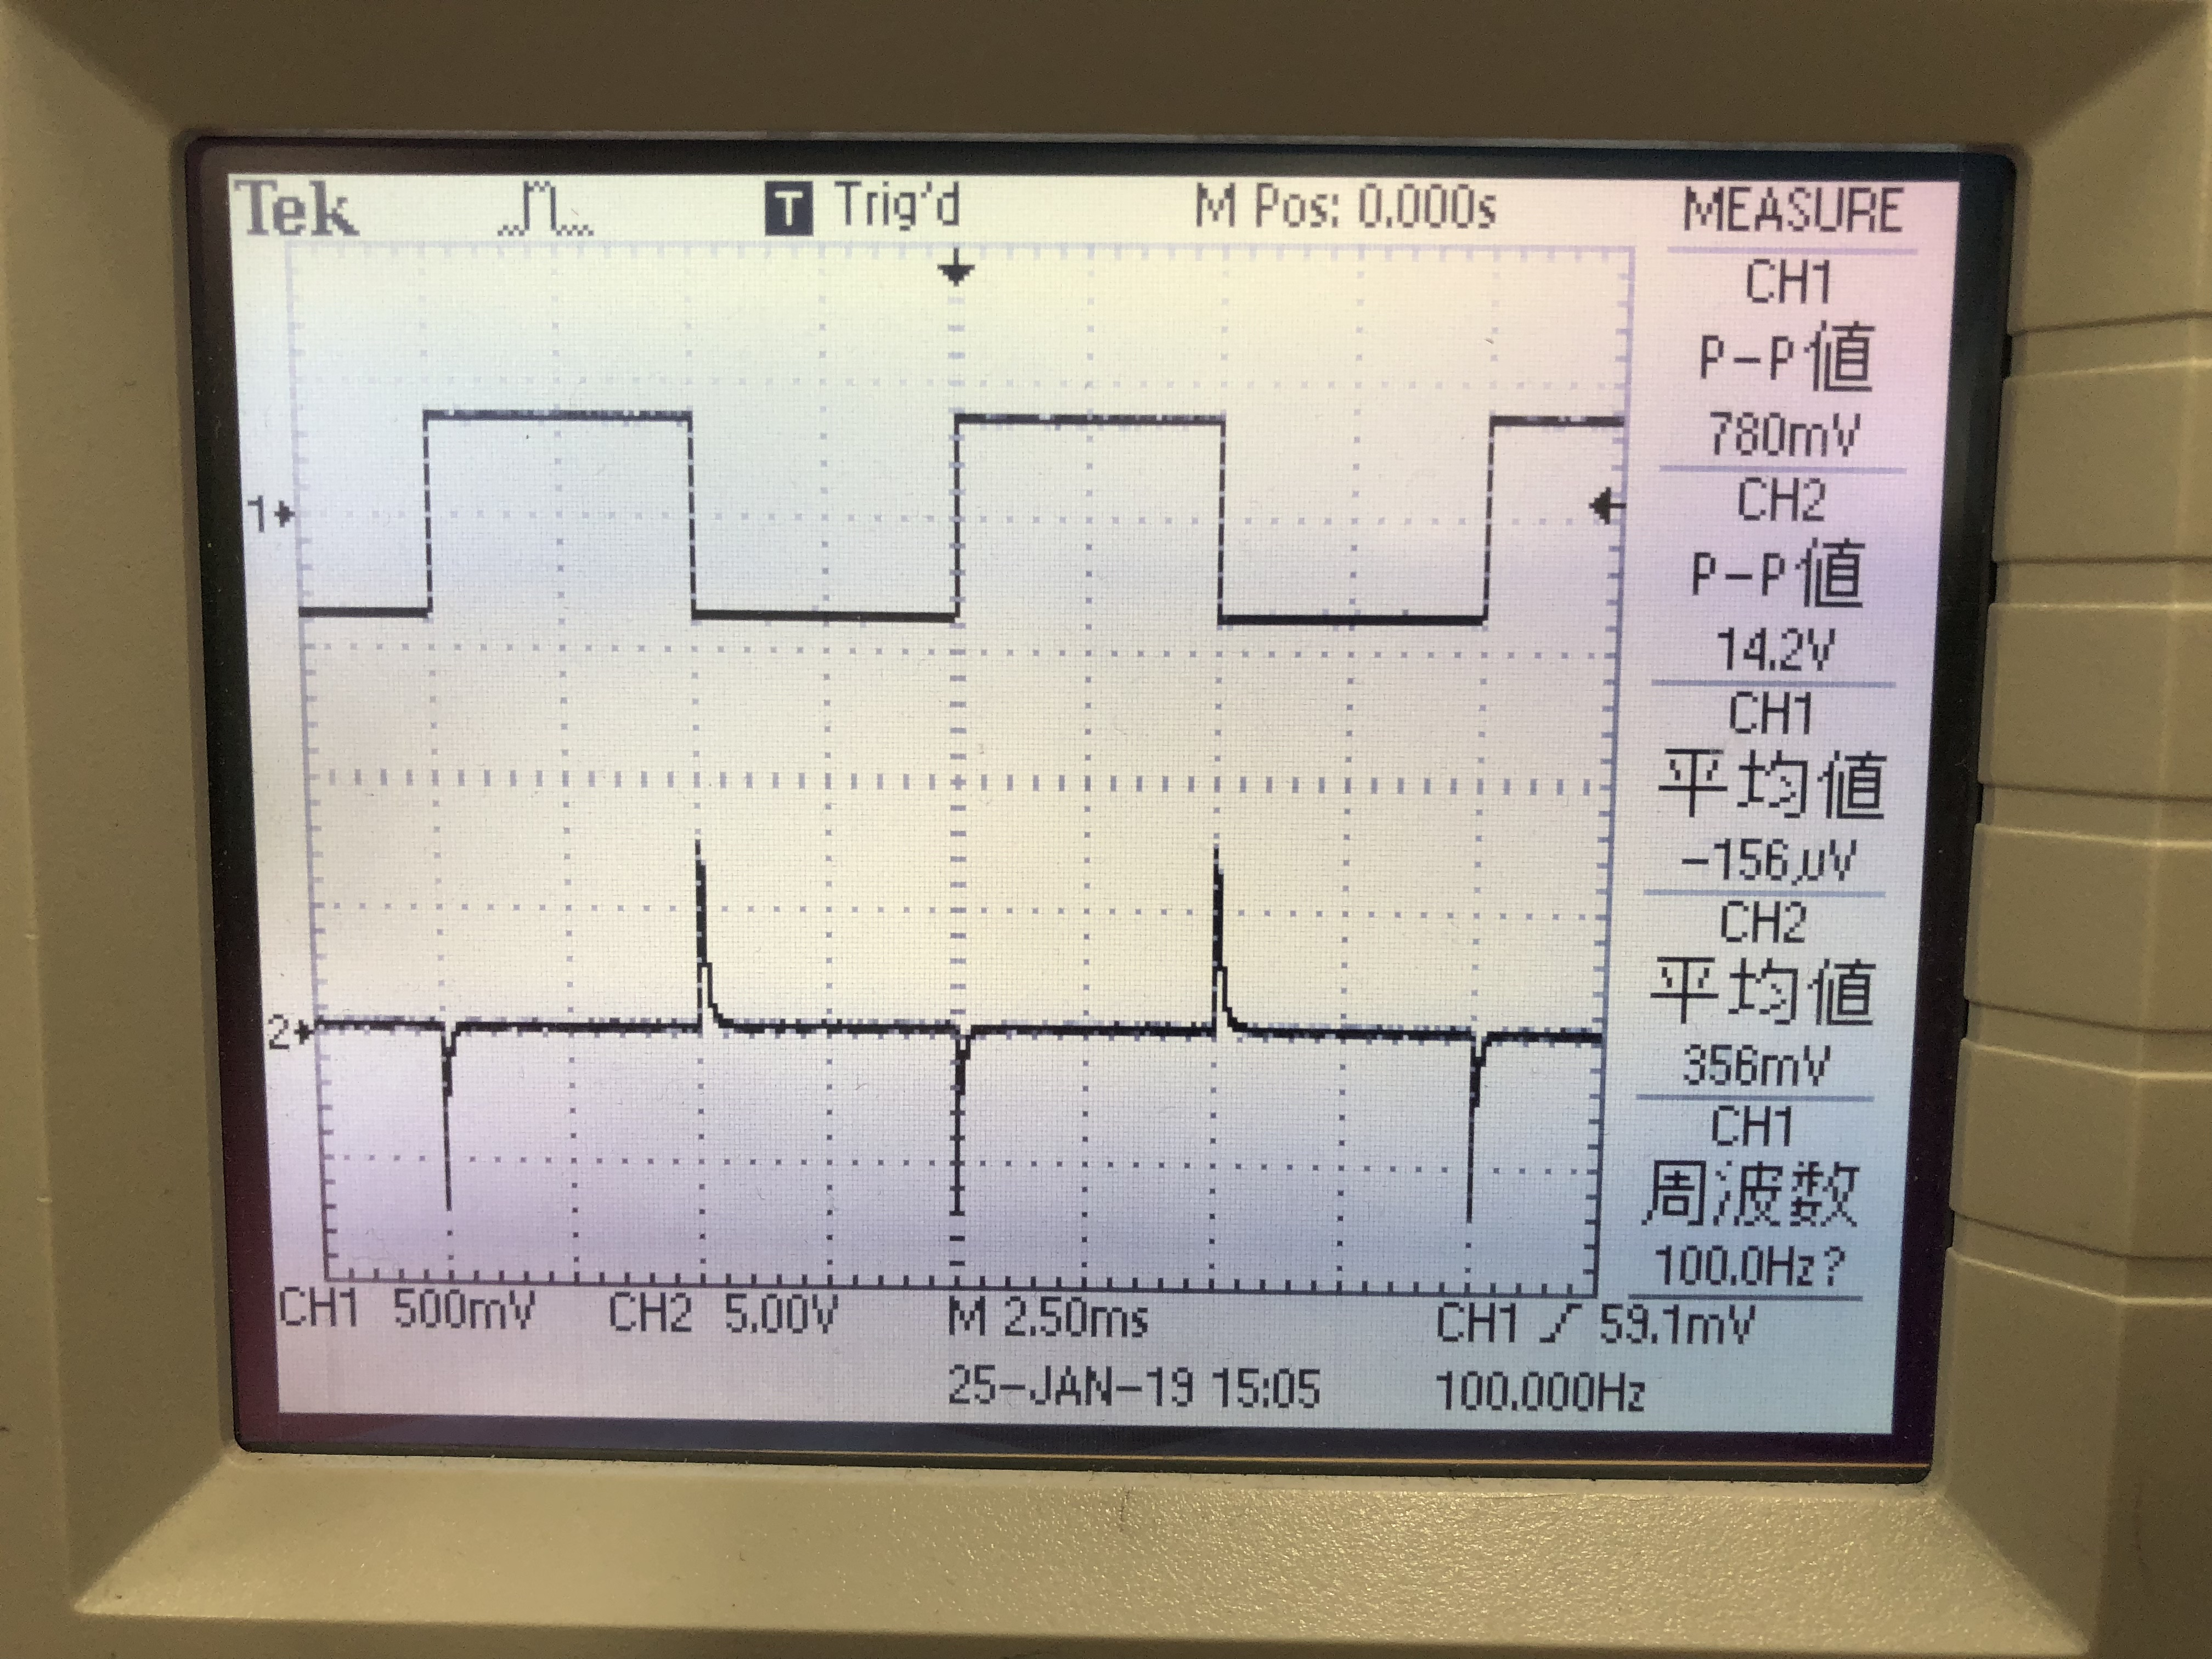
\includegraphics[width=7cm]{../img/result_bibun_100hz.jpg}
                \caption{100Hzにおける微分回路の可視化結果.}
            \end{center}
          \end{figure}


          \begin{figure}[]
            \begin{center}
                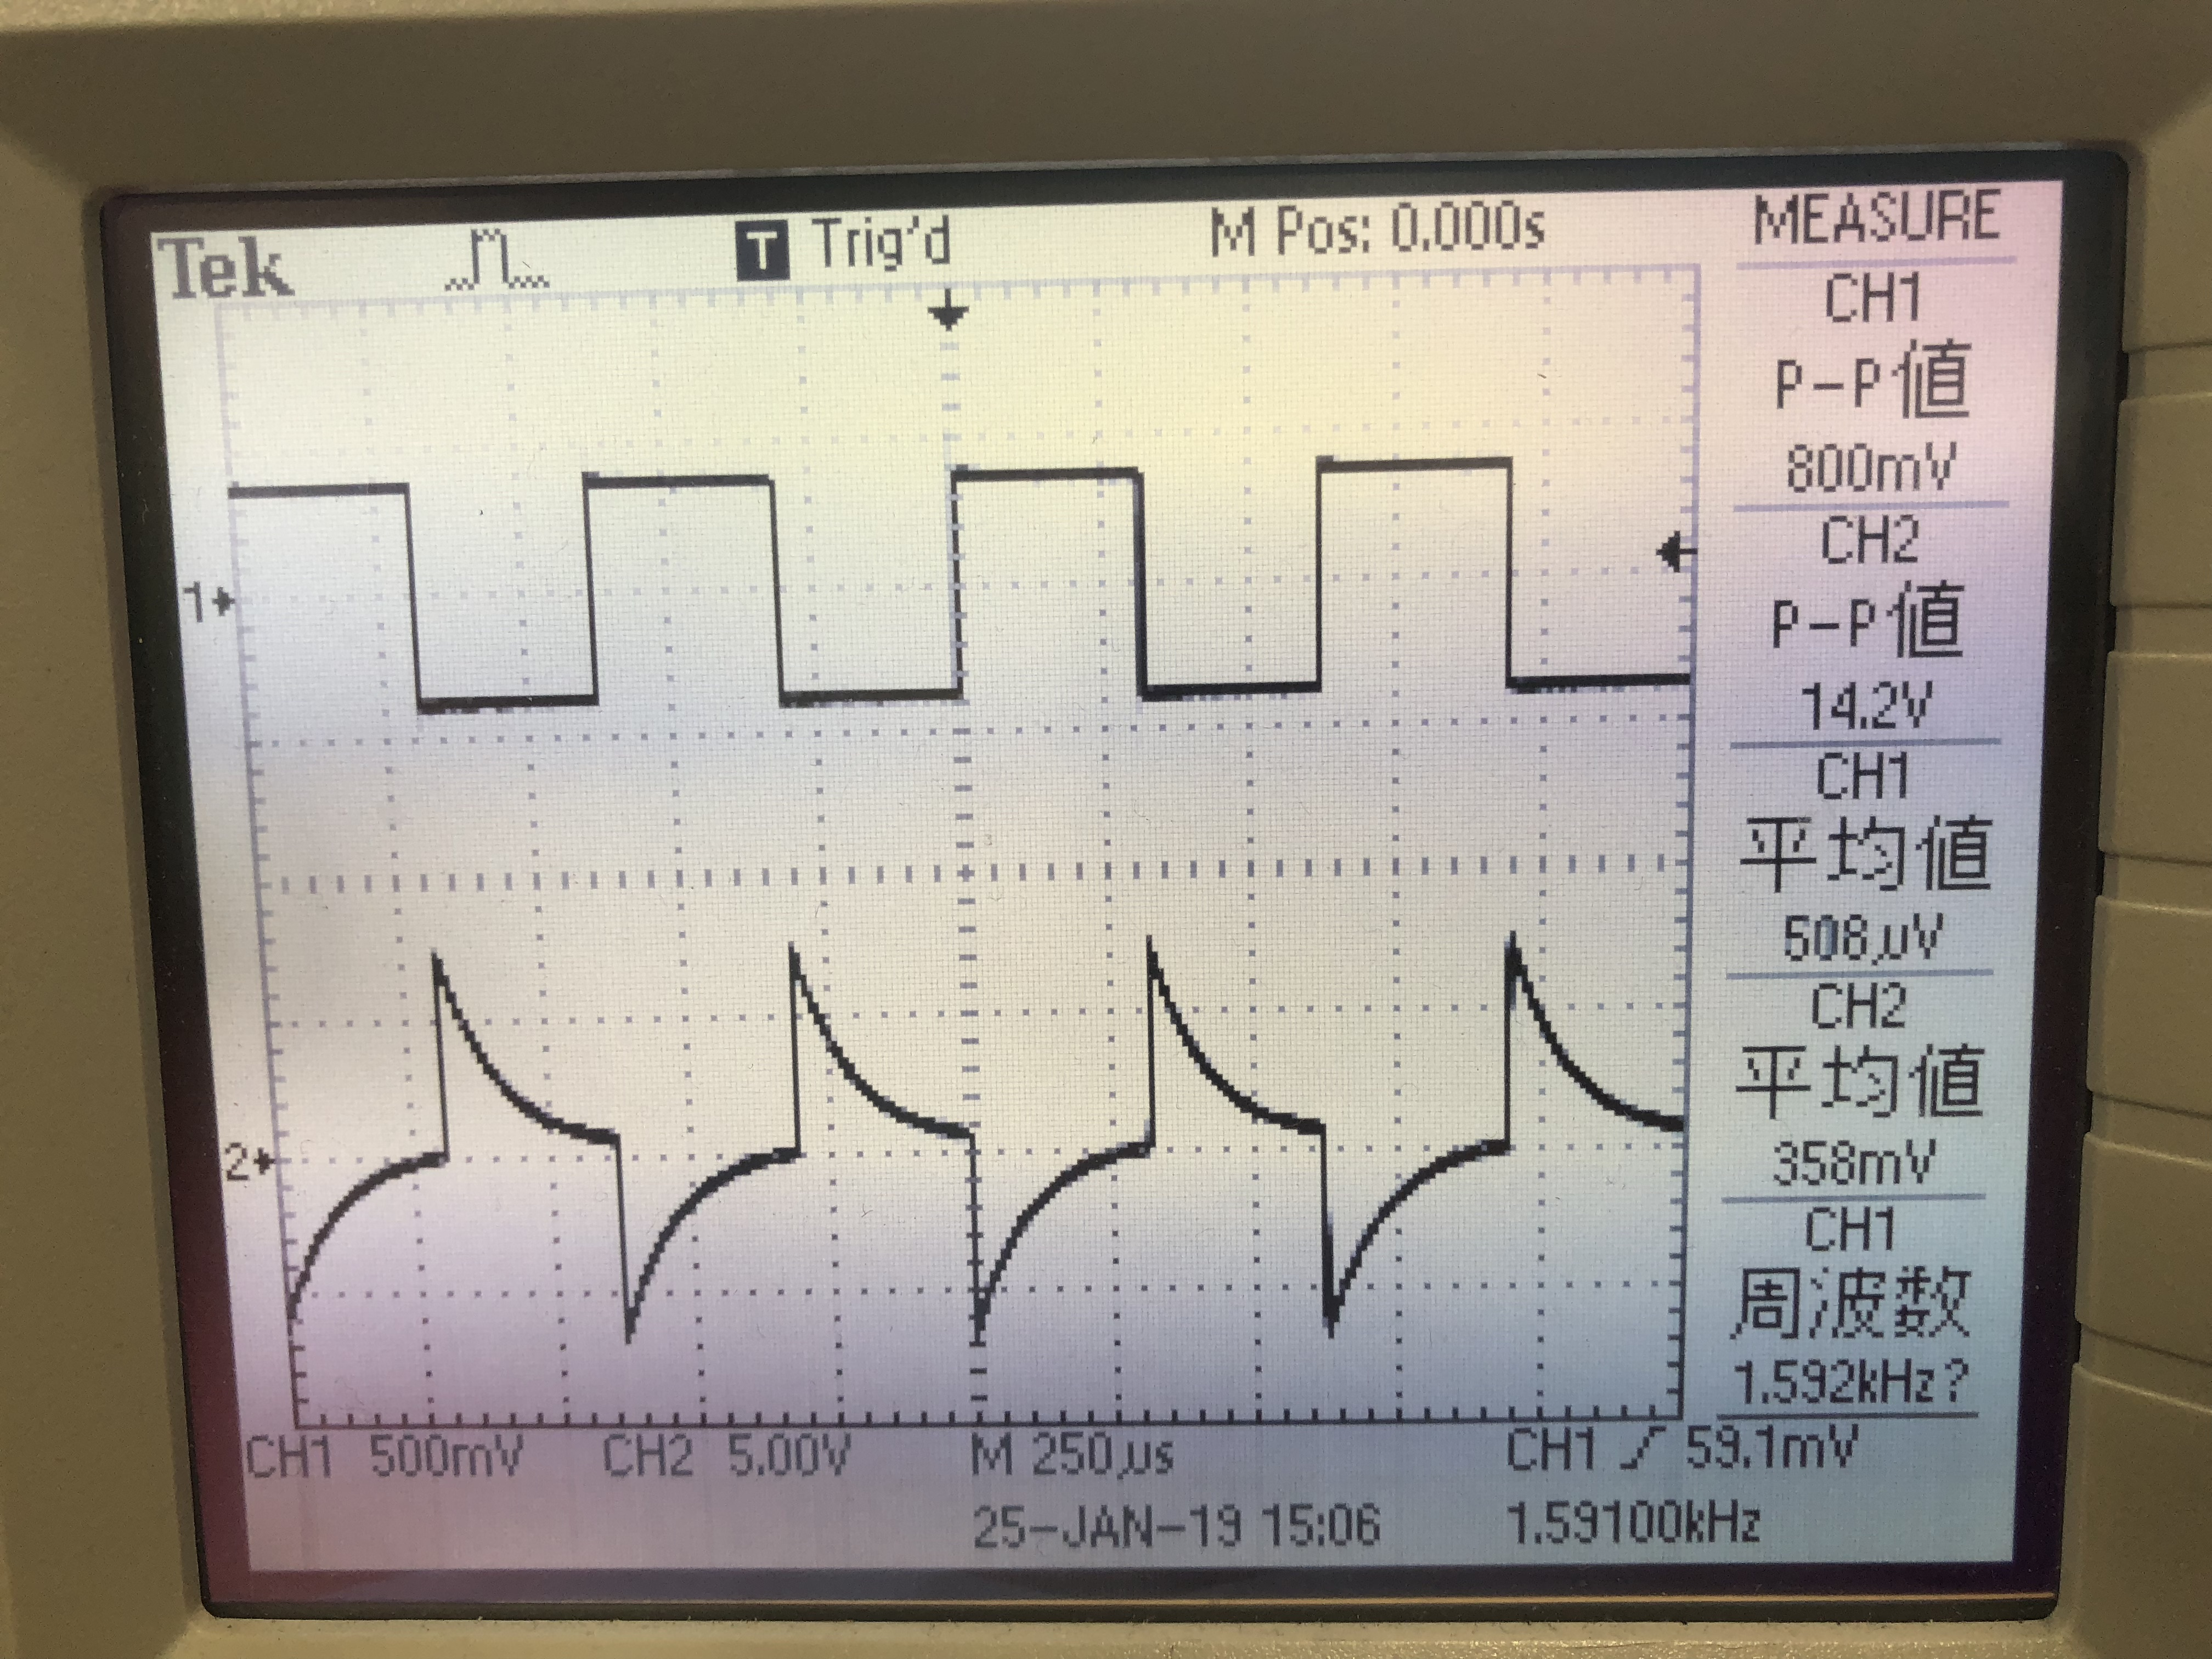
\includegraphics[width=7cm]{../img/result_bibun_1500hz.jpg}
                \caption{1500Hzにおける微分回路の可視化結果.}
            \end{center}
          \end{figure}


          \begin{figure}[]
            \begin{center}
                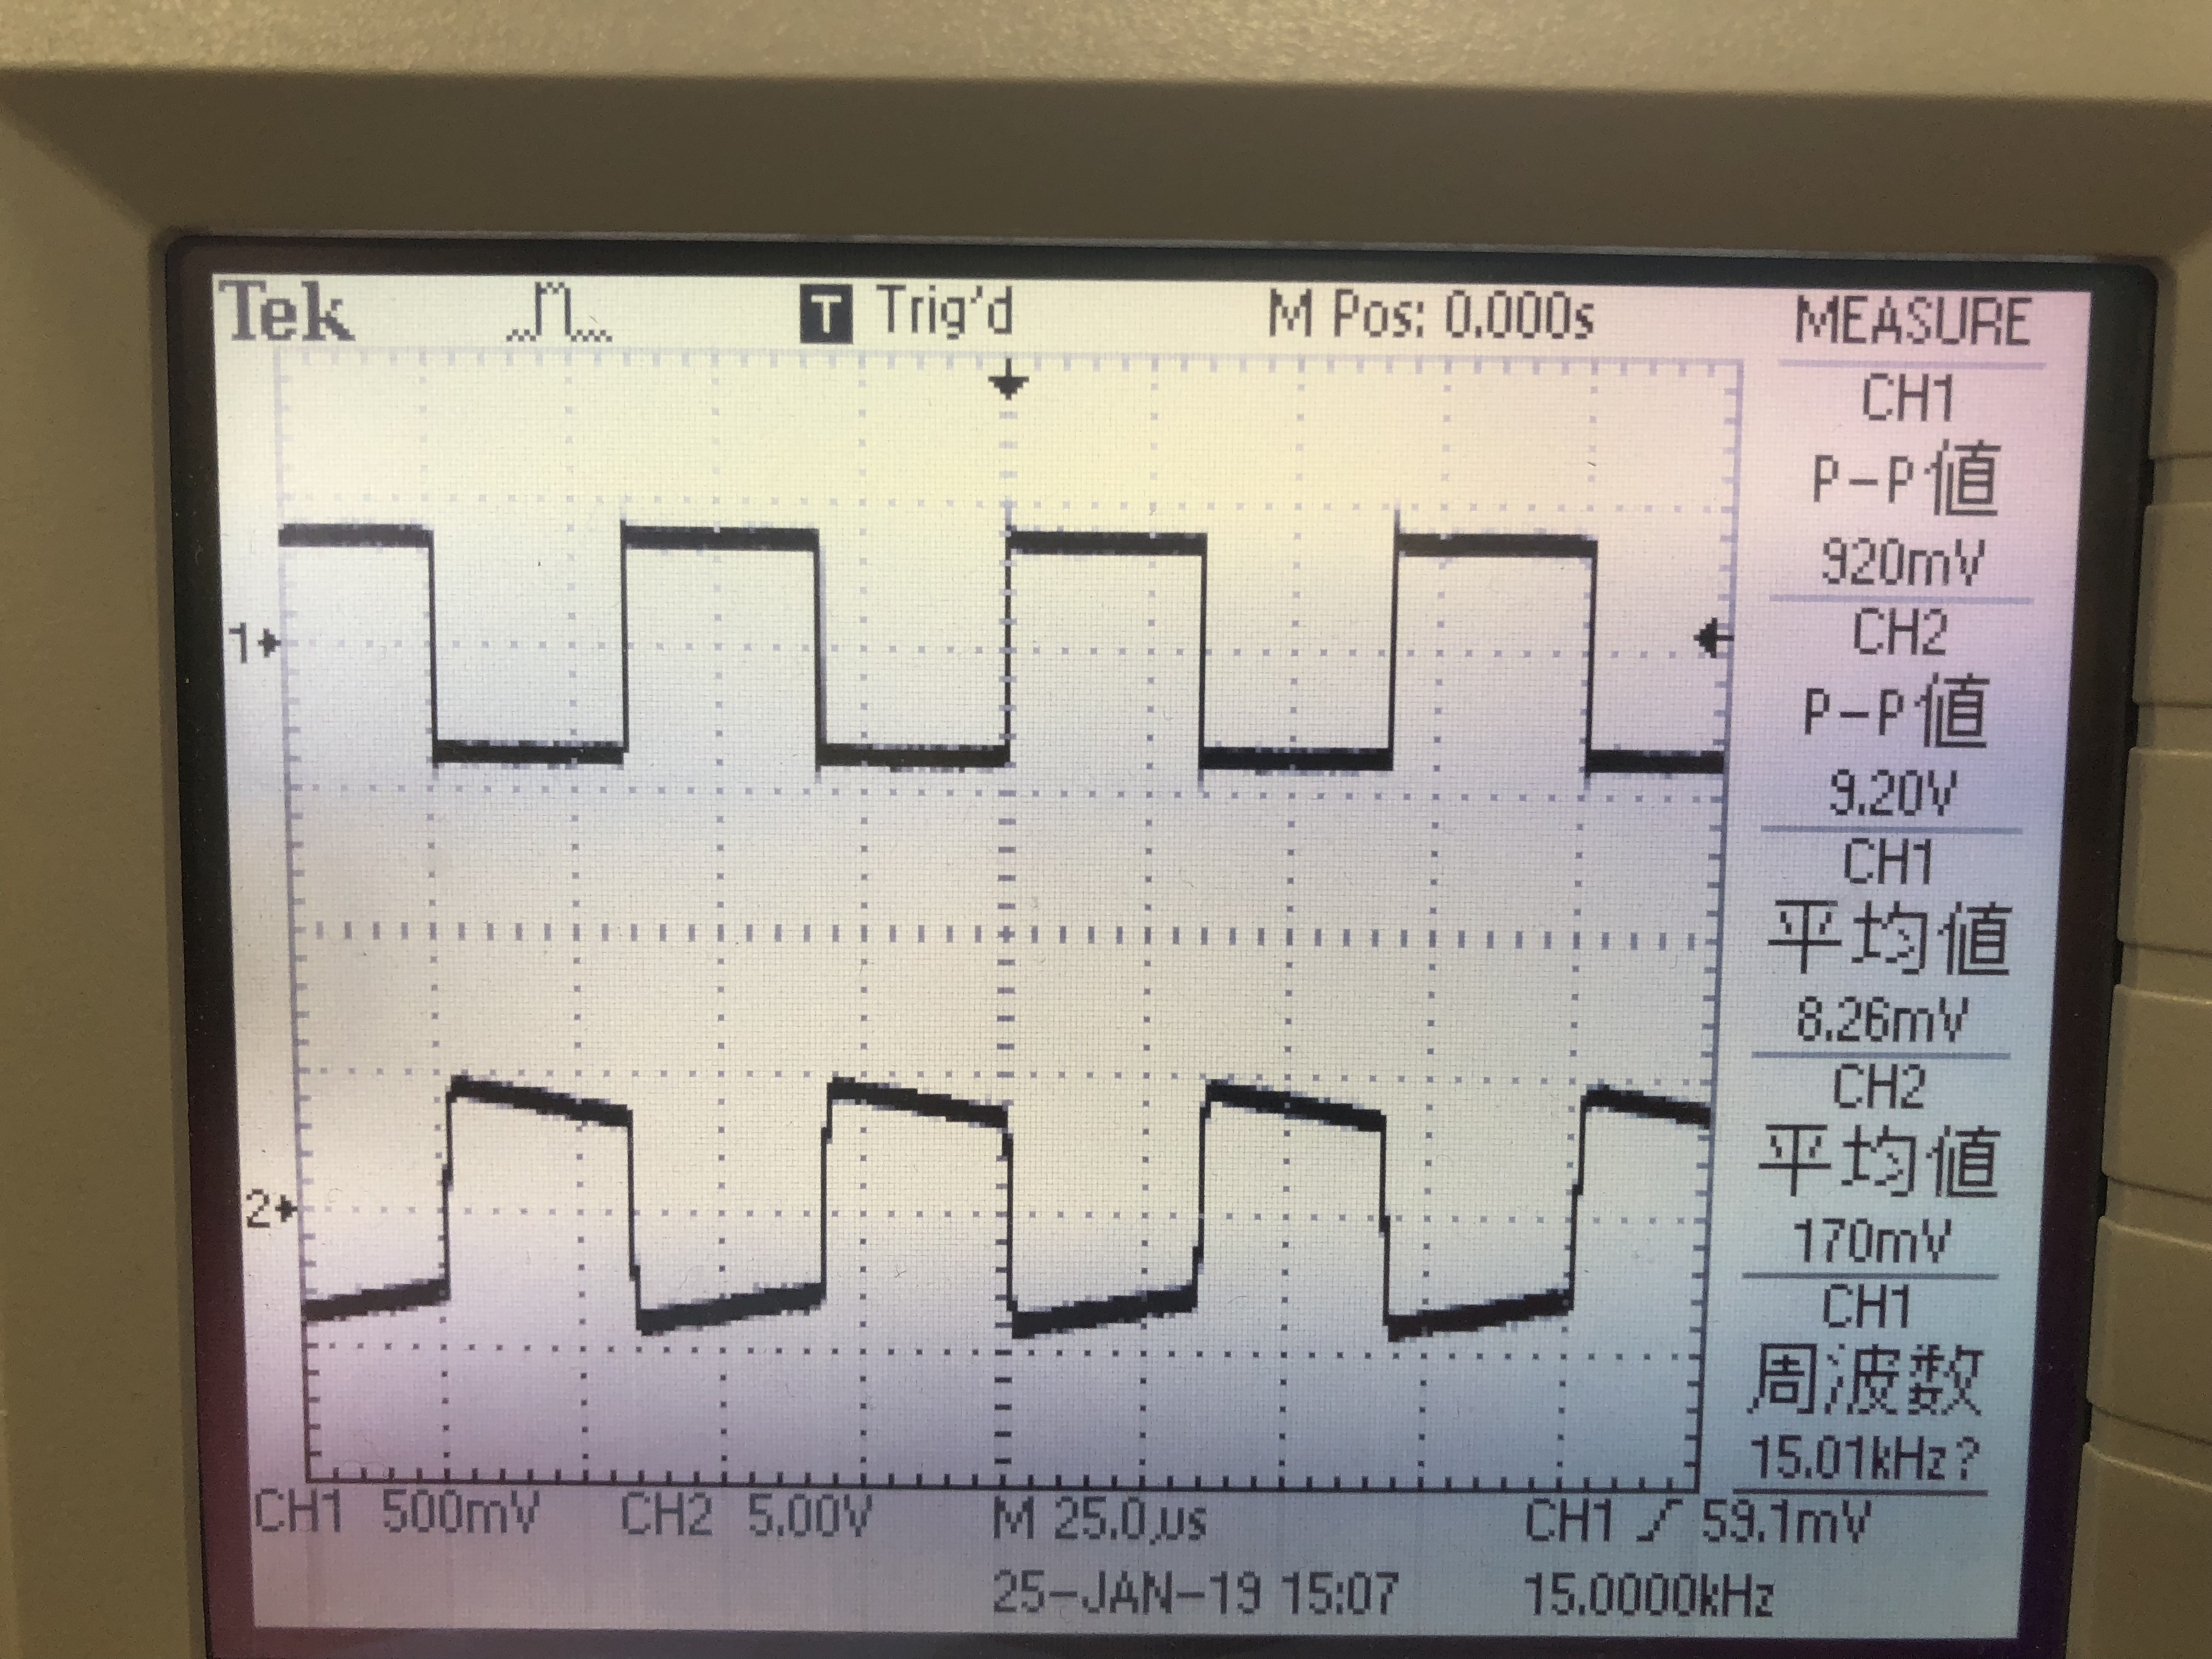
\includegraphics[width=7cm]{../img/result_bibun_15000hz.jpg}
                \caption{150000Hzにおける微分回路の可視化結果.}
            \end{center}
          \end{figure}


        
        \subsection{積分回路}
        測定結果を,表9,図18,19,20に示した.

        \begin{table}[H]
          \centering
          \footnotesize
          \caption{積分回路の抵抗,静電容量,$f_{s}$の値.}
          \label{opeanpu_risouteki_tokusei}
          \begin{tabular}{llll} \hline
            $R_{1} k\Omega$ & $R_{2} k \Omega$& $C_{1} \mu F$& $f_{0} Hz$ \\ \hline
            10	&200	&0.0011	&723.431 \\ \hline 
          \end{tabular}
        \end{table}

        \begin{figure}[]
          \begin{center}
              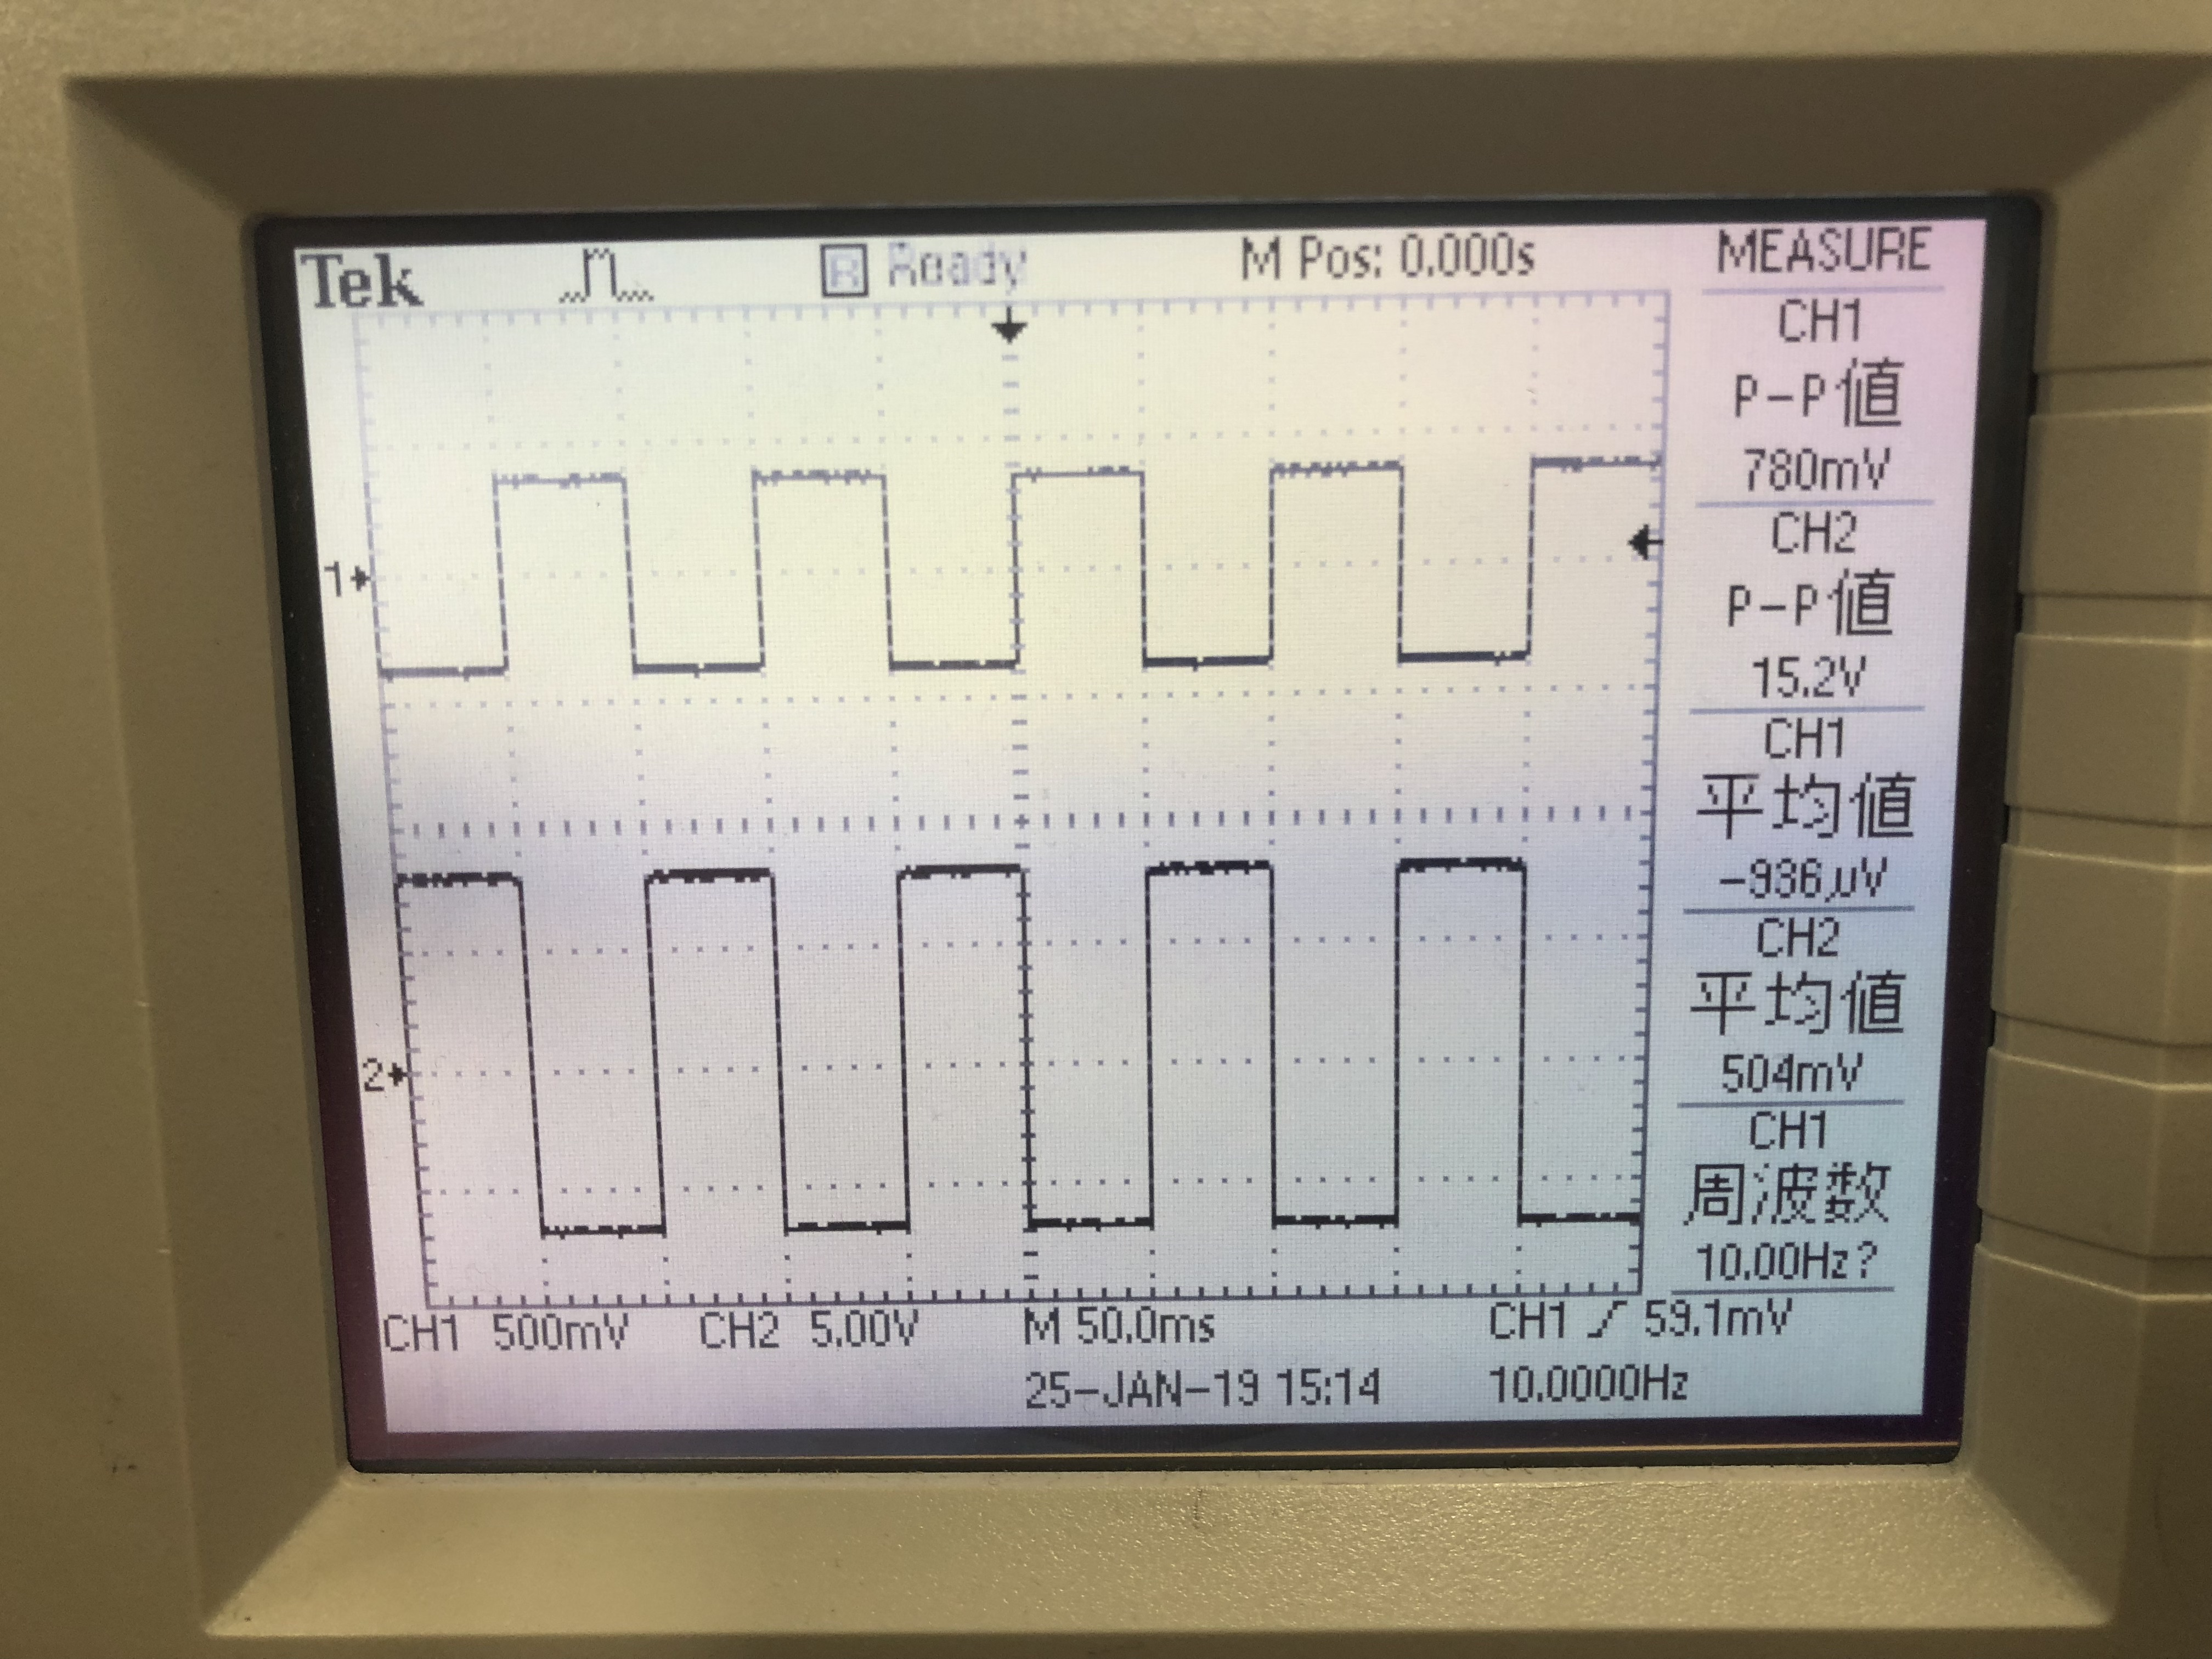
\includegraphics[width=7cm]{../img/result_sekibun_10Hz.jpg}
              \caption{10Hzにおける積分回路の可視化結果.}
          \end{center}
        \end{figure}

        \begin{figure}[]
          \begin{center}
              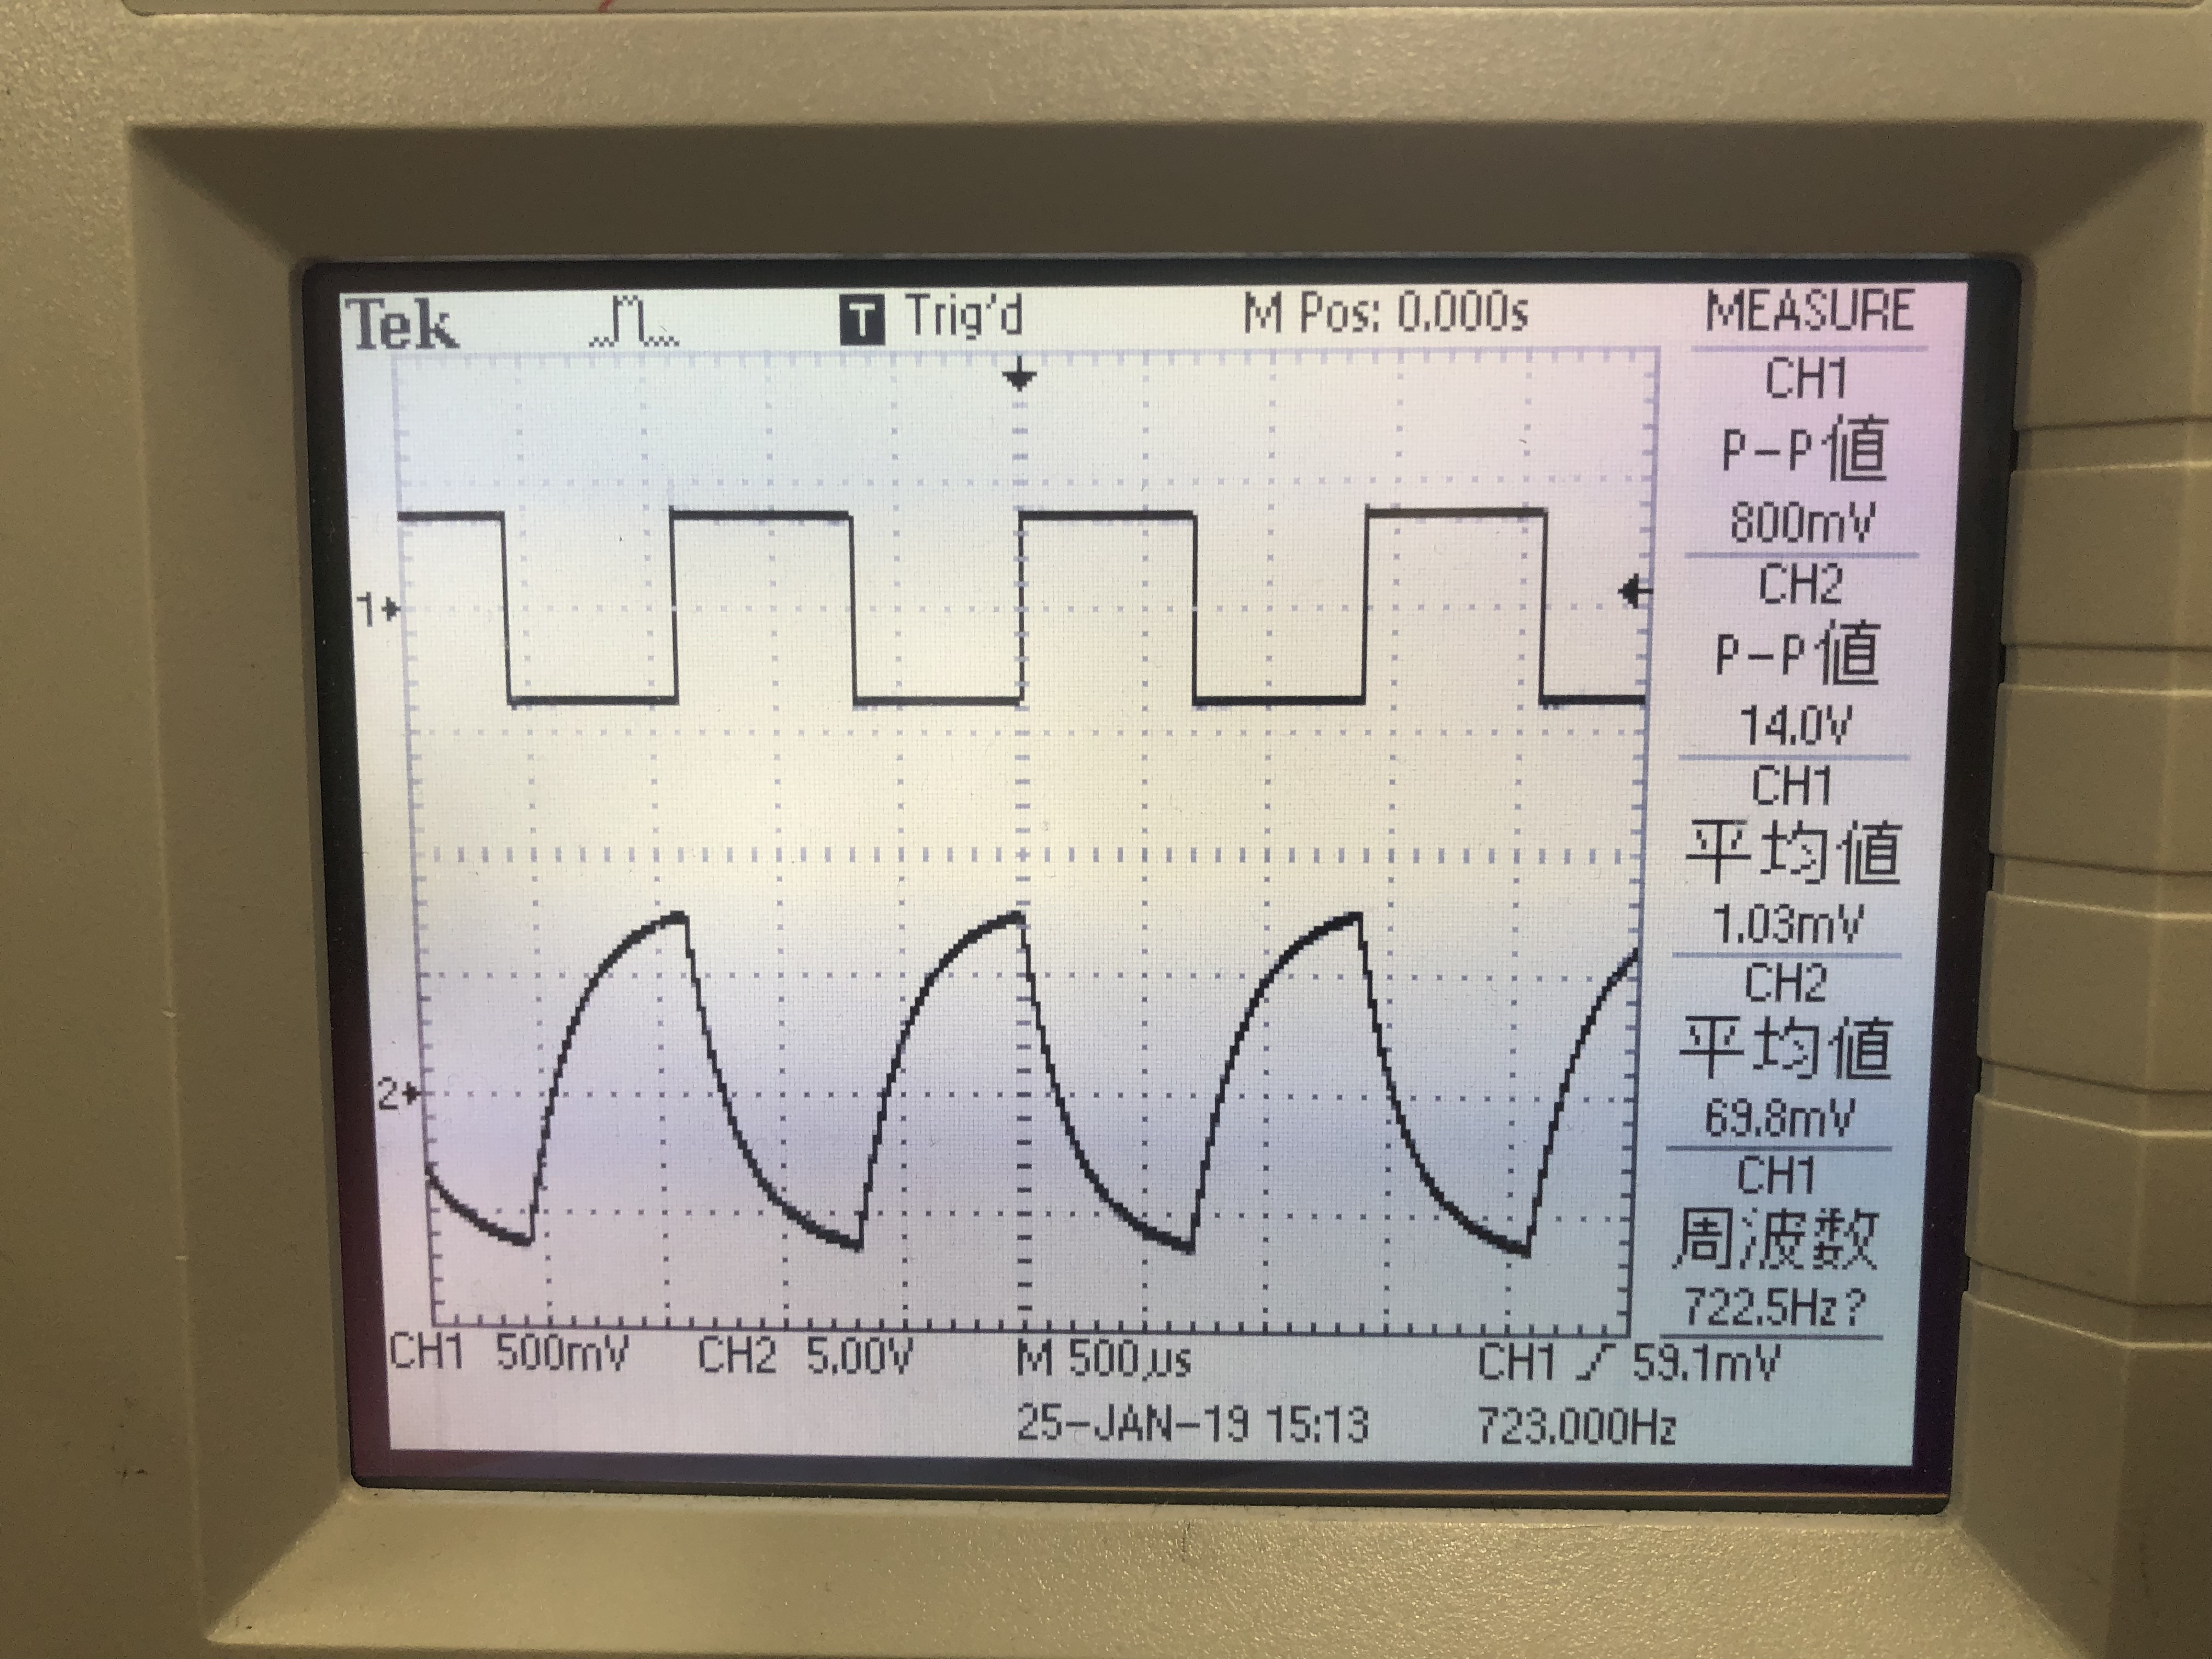
\includegraphics[width=7cm]{../img/result_sekibun_700Hz.jpg}
              \caption{700Hzにおける積分回路の可視化結果.}
          \end{center}
        \end{figure}

        \begin{figure}[]
          \begin{center}
              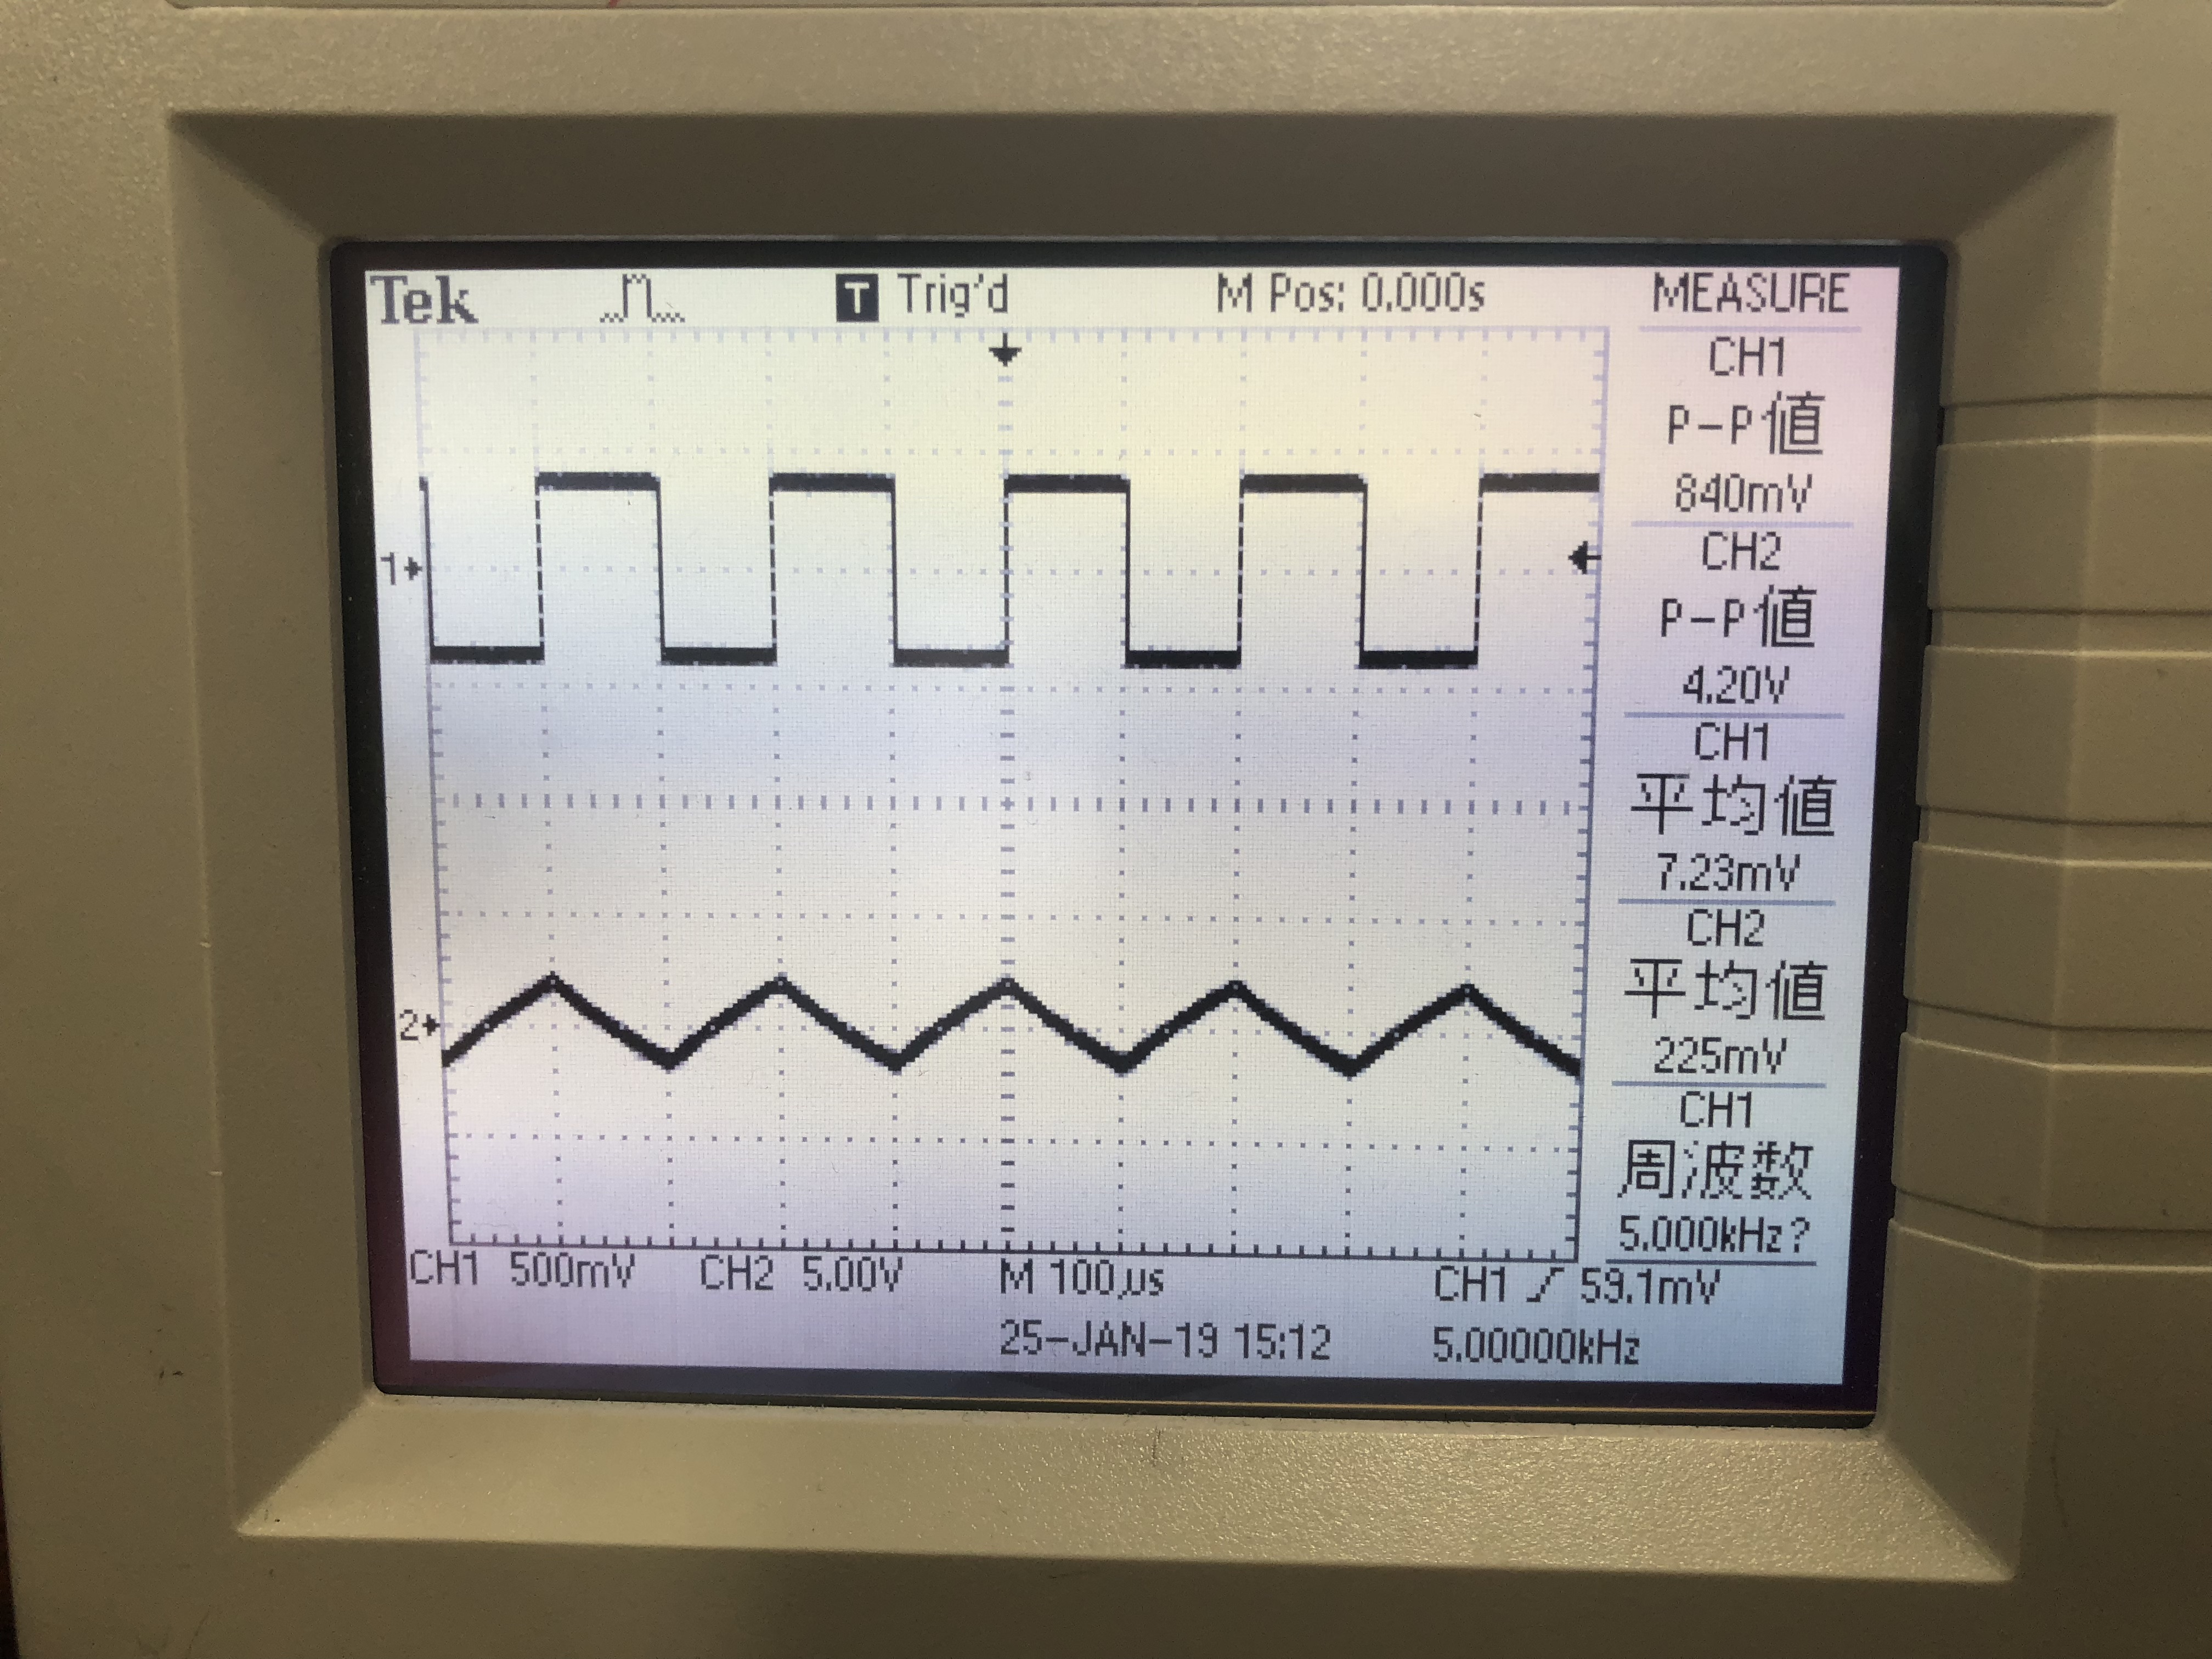
\includegraphics[width=7cm]{../img/result_sekibun_5000Hz.jpg}
              \caption{5000Hzにおける積分回路の可視化結果.}
          \end{center}
        \end{figure}

\section{考察}
% 考察
      \subsection{反転増幅回路の理論増幅度と実際との比較}
        理論電圧増幅度$A=-1$のとき,$V_{i} = 0.000002$Vのとき以外は電圧増幅度$A$が1.16から0.85
        の範囲に収まっており,実験結果と理論値の誤差はあるものの想定される結果が得られた.

        また,理論電圧増幅度$A=-10$のとき,$V_{i} = 0$Vのとき以外は,$A$が12から4.13と理論値からは大きくずれた部分も見られた.
        これは,オペアンmぷの出力電圧は電源電圧に依存するため,出力電圧が電源電圧と入力電圧の和以上になることができないためである.
        図8より上限や下限が実際に見られた. 

      \subsection{反転増幅回路の動作周波数}
        周波数が20KHz程度までは,理論電圧増幅度$G = 20$dBに近い電圧増幅度であり,
        この値を越えると,少しずつ減少し,100Hzを超えたあたりから急激に減少していった.


        これは,周波数が大きくなっていくにつれ,オペアンプのスルーレートの関係[2]を満たさなくなったからだと考えられる.

      \subsection{反転・非反転増幅回路の特徴と相違点}
        反転増幅回路では,出力電圧と入力電圧の極性が逆になるが,非反転増幅回路では等しくなる.
        また,回路中で用いる抵抗値が同じならば,電圧増幅度の絶対値は非反転増幅回路の方が大きくなる.


        相違点としては,反転増幅回路では,正相入力端子をグラウンドに接地させるが,非反転増幅回路では,
        逆正相入力端子をグラウンドに接地させる[3].

      \subsection{各フィルタの理論周波数特性と実測周波数特性の比較およびカットオフ周波数について}
        ローパスフィルタ回路のカットオフ周波数は,実測値は約60Hzであり,理論値は約60Hzであった.
        ハイパスフィルタ回路は,実測値は約900Hzであり,理論値は約1000Hzであった.
        誤差が生じた理由は,実際に回路を用いて実験をすると流している電圧の損失があったりしたためだと
        考えられる.
        理論値と実測値を比較した図を21,22に示す.
      
      \subsection{微分・積分回路}
        出力される波形は,微分回路では図15-16より微分された値の反転,積分回路では図17-20より
        積分された値が反転したものが得られている. しかし,微分回路においては図16,17,積分回路においては
        図18で正しく結果が得られなかった. つまり,微分回路では$f < f_{s}$,積分回路では$f>f_{s}$において
        正しい波形が観測できることがわかった.




        \begin{figure}[]
          \begin{center}
              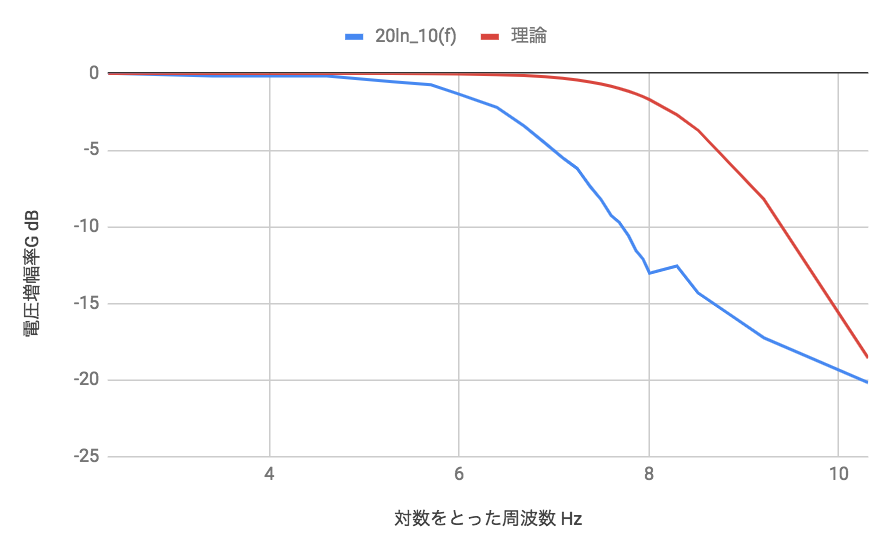
\includegraphics[width=7cm]{../img/result_riron_low.png}
              \caption{ローパスフィルタの理論値と実測値の比較.}
          \end{center}
        \end{figure}

        \begin{figure}[]
          \begin{center}
              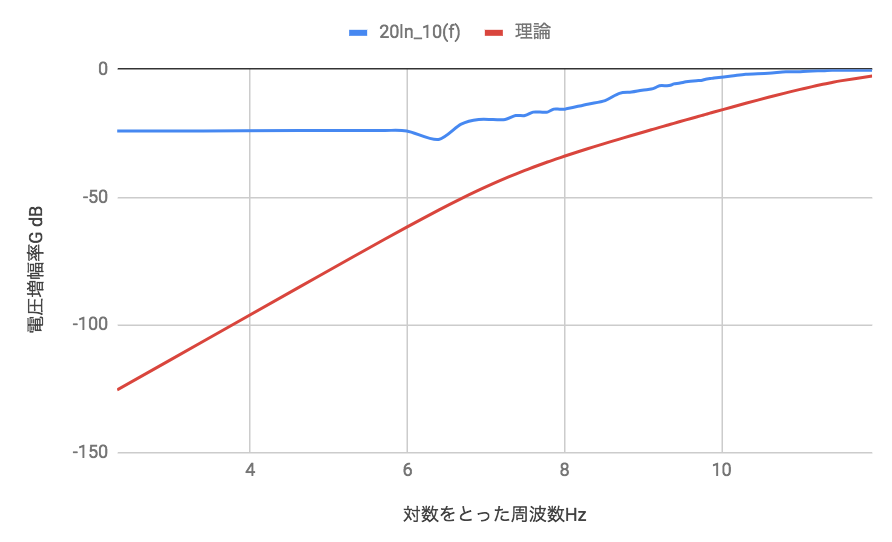
\includegraphics[width=7cm]{../img/result_riron_high.png}
              \caption{ハイパスフィルタの理論値と実測値の比較.}
          \end{center}
        \end{figure}
        

        


\begin{thebibliography}{3}
\bibitem{}Wikipedia 微分回路 https://ja.wikipedia.org/wiki/ \\ \%E5\%BE\%AE\%E5\%88\%86\%E5\%9B\%9E\%E8\%B7\%AF

\bibitem{}ローム株式会社 スルーレート https://www.rohm.co.jp/electronics-basics/opamps/op\_what5  
\bibitem{}北海道大学 電子工学実験I(2000年~2006年)演算増幅器を用いた基本回路 https://www.rohm.co.jp/electronics-basics/opamps/op\_what5  

https://ime.ist.hokudai.ac.jp/~aoki/laboratory02.html

\bibitem{}電気通信大学 共通教育部自然科学部会(物理) :基礎科学実験A p73-79
\end{thebibliography}
\end{document}